%   % !TEX root = ../../VIII,3_Rahmen-TeX_9-0.tex
%  
%   Band VIII, 3		Rubrik STOSS
%
%   Signatur/Tex-Datei:	LH_38_212-215
%
%   RK-Nr. 	55822		
%
%   Überschrift: 	Elemens de Mecanique...
%   
%   Unterrubrik:			Auszüge
%
%
%	WZ:		LEd8-WZ 803043 in 213
%			LEd8-WZ 803013 in 214-215
%
%   edlabels:			28
%
%   Diagramme: 		15		(wieviele?)			
%
%
%   NB: 						(Anmerkungen)					??
%
%
%
\selectlanguage{ngerman}
\frenchspacing
%
\begin{ledgroupsized}[r]{120mm}
\footnotesize
\pstart
\noindent\textbf{Überlieferung:}
\pend
\end{ledgroupsized}
%
\begin{ledgroupsized}[r]{114mm}
\footnotesize
\pstart \parindent -6mm
\makebox[6mm][l]{\textit{L}}%
Auszüge mit Bemerkungen 
aus \protect\index{Namensregister}{\textso{Parent}, Antoine 1666\textendash1716}A.~\textsc{Parent}, \cite{01500}\textit{Élémens de méchanique et de physique}, Paris 1700: 
LH~XXXVIII Bl.~212\textendash215.
Zwei Bogen 2\textsuperscript{o} (Bl.~212\textendash213 und Bl.~214\textendash215); ein Wasserzeichen in Bl.~213 sowie ein weiteres Wasserzeichen in Bl.~214 mit Gegenmarke in Bl.~215. Sieben Seiten; Bl.~215~v\textsuperscript{o} leer.
Textfolge durch den eigh.\ Ordnungsvermerk \glqq 2.\grqq\ am Anfang des zweiten Bogens (Bl.~214~r\textsuperscript{o}) gesichert;
auf Bl.~214~r\textsuperscript{o} und Bl.~215~r\textsuperscript{o} je ein gestrichener Diagrammentwurf, die nicht wiedergegeben werden.
\pend
\end{ledgroupsized}
%
%
%
%
\selectlanguage{french}
\frenchspacing
% \newpage%
\vspace{8mm}
\pstart%
\normalsize%
\noindent%
\lbrack212~r\textsuperscript{o}\rbrack\
\pend
%
% Überschrift
\count\Bfootins=1200%
\count\Afootins=1200%
\count\Cfootins=1200 
\pstart
\centering
%
\cite{01500}\textit{Elemens de Mecanique et de physique où l'on donne geometriquement les principes du choc et des equilibres entre toutes sortes de corps; avec l'explication naturelle des machines fondamentales} 
par Monsieur 
A.~Parent\protect\index{Namensregister}{\textso{Parent}, Antoine 1666\textendash1716} 
de l'Académie Royale des sciences.\protect\index{Sachverzeichnis}{Académie Royale des Sciences} Paris 
\edtext{chez Delaulne}{\lemma{chez}\Bfootnote{\textit{(1)} de l \textit{(2)} Delaulne \textit{L}}} 
%
1700 in 8\textsuperscript{o}.\ pagg.~449. 
\pend
\vspace{0.5em}
%
\pstart\noindent
%
\textso{Preface}.
%
\edtext{\textit{Ayant trouvé que la maniere de rappeller tous les chocs\protect\index{Sachverzeichnis}{choc} à l'equilibre ou de les en deduire par des}
%
\edtext{\textit{temoins} \lbrack\textit{auxiliaires}\rbrack, contenoit}{\lemma{\textit{temoins}}\Bfootnote{\textit{(1)} anulaires \textit{(2)} \textbar\  oculaires \textit{ändert Hrsg. nach Vorlage} \textbar\ , \textit{contenoit} \textit{L}}} 
%
\textit{la connoissance de tout ce qu'on peut desirer du mouvement, et croyant que ce fut une chose tout a fait nouvelle je m'appliquay l'annee derniere à pousser cette methode\dots}}{\lemma{\textit{Ayant trouvé}  \lbrack...\rbrack\ \textit{cette methode}}%
\Cfootnote{\protect\index{Namensregister}{\textso{Parent}, Antoine 1666\textendash1716}A.~\textsc{Parent}, \cite{01500}\textit{Élémens de méchanique et de physique}, Paris 1700, Preface, S.~\lbrack 1\rbrack.}}
%
\edtext{\textit{Depuis que ce traité est achevé on m'a fait voir plusieur auteurs, comme Messieurs 
Wallis\protect\index{Namensregister}{\textso{Wallis} (Wallisius), John 1616\textendash1703}, et 
Mariotte\protect\index{Namensregister}{\textso{Mariotte}, Edme, Seigneur de Chazeuil ca. 1620\textendash1684} 
dans son Traité de la percussion, 
qui semblent avoir en vuë la même maniere de considerer le mouvement, 
quoyqu'ils ne se soyent pas expliqués de même, si ce n'est peut estre M.~Mariotte\protect\index{Namensregister}{\textso{Mariotte}, Edme, Seigneur de Chazeuil ca. 1620\textendash1684} 
dans ses mouvemens composés\protect\index{Sachverzeichnis}{mouvement composé}. On m'a asseuré de plus que}
%
\edtext{\textit{M. Huguens}\protect\index{Namensregister}{\textso{Huygens} (Hugenius, Ugenius, Hugens, Huguens), Christiaan 1629\textendash1695}}{\lemma{\textit{M}.}\Bfootnote{\textit{(1)} Hugen \textit{(2)} \textit{Huguens} \textit{L}}} 
%
\textit{avoit publié dès longtemps ce même principe dans plusieurs} 
%
\edtext{\textit{journaux.}}{\lemma{}\Afootnote{\foreignlanguage{ngerman}{\textit{Am Rand}:} \textasteriskcentered\ luy signifie la multiplication.\textsuperscript{\lbrack a\rbrack}
\newline\vspace{-0.5em}\newline%Marginalienapparat:
{\footnotesize
\foreignlanguage{ngerman}{\textsuperscript{\lbrack a\rbrack} \textasteriskcentered\ \lbrack...\rbrack\ multiplication: a.a.O., Avertissement, S.~\lbrack 9\rbrack.}\vspace{-3mm}%
}}}
%
\textit{Cependant le peu de progrés, qu'on}
%
\textit{a fait jusqu'icy dans la connoissance du choc, me pourroit faire croire que la maniere d'en faire} l'\textit{application, n'a pas encor esté} 
%
assez \textit{connue, puisqu'encor aujourdhuy plusieurs Auteurs celebres ont leurs principes particuliers, et sont si peu d'accord entre eux.}
%
\textit{Si je me} trouve \textit{redevable à quelcun de quelque chose, ce ne peut estre qu'aux ouvrages de Messieurs \protect\index{Namensregister}{\textso{Renau d'Eli\c{c}agaray}, Bernard, 1652\textendash1719}Renaut sur la manoeuvre,
Mariotte\protect\index{Namensregister}{\textso{Mariotte}, Edme, Seigneur de Chazeuil ca. 1620\textendash1684}
sur les}
%
\edtext{\textit{liqueur}\lbrack\textit{s}\rbrack}{\lemma{}\Bfootnote{liqueur \textit{L ändert Hrsg.\ nach Vorlage}}}, 
%
\textit{et de la Hire\protect\index{Namensregister}{\textso{La Hire}, Philippe de 1640\textendash1718} 
sur la Mecanique. Mais je reconnois l'estre par dessus tout aux lumieres de ce sçavant et illustre genie}
%
\textit{Monsieur Sauveur,\protect\index{Namensregister}{\textso{Sauveur}, Joseph 1653\textendash1716} dont la seule modestie m'empeche de m'étendre d'avantage sur son merite infini dans les Mathematiques et dans la physique\dots}}{\lemma{\textit{Depuis que}  \lbrack...\rbrack\ \textit{la physique}}\Cfootnote{a.a.O., S. \lbrack 3\textendash5\rbrack\ mit Auslassungen.\cite{01500}}}
%
\edtext{\textit{On ne demande autre}
%
\edtext{\lbrack\textit{chose que}\rbrack}{\lemma{}\Bfootnote{che \textit{L ändert Hrsg. nach Vorlage}}} 
%
\textit{de s'imaginer ce qui paroistroit si estant sur le rivage d'une riviere, ils regardoient des personnes jouer à la boule, dans un vaisseau\protect\index{Sachverzeichnis}{vaisseau} emporté par le courant de la riviere;}  
\textit{ou} \textit{qu'ils fassent construire une machine semblable à celle qui est à la fin de ce livre.}
\textit{Alors} \textit{ils apprendront par eux mêmes ce grand principe de la nature, que le mouvement n'est rien de positif}.}{%
\lemma{\textit{On ne}  \lbrack...\rbrack\ \textit{de positif}}
\Cfootnote{a.a.O., S. \lbrack 5\rbrack\ mit Auslassungen.\cite{01500}}}
\pend
\count\Bfootins=1200%
\count\Afootins=1200%
\count\Cfootins=1200 
%
\pstart
\hspace{1mm}\hspace{-1mm}% Trick, weil \edlabel nicht zu \par-Beginn sein darf
\edlabel{38_212-215_212r1}%	
\edtext{}{{\xxref{38_212-215_212r1}{38_212-215_212r2}}\lemma{\textit{Quant au} \lbrack...\rbrack\ \textit{de gravité}}\Cfootnote{a.a.O., S. \lbrack 6f.\rbrack\ mit Auslassungen.\cite{01500}}}%
%
\textit{Quant au titre du livre,} \textit{la physique n'est qu'un pur effect du choc des corps,} 
ainsi les \textit{Elemens du choc} sont ceux \textit{de toute la physique}. \pend
%
\pstart 
%
\textit{On trouvera} \textit{un principe nouveau du choc composé\protect\index{Sachverzeichnis}{choc composé},} \textit{que j'ay substitué} à \textit{celuy des parallelogrammes, qui quoyqu'il soit veritable dans les équilibres autour d'un point fixe, conduit cependant infalliblement à l'erreur dans les chocs libres\protect\index{Sachverzeichnis}{choc libre}, 
comme il est aisé de le voir, quand on veut passer du choc composé}
%
\edtext{\lbrack \textit{au}\rbrack}{\lemma{}\Bfootnote{aux \textit{L ändert Hrsg. nach Vorlage}}} 
%
\textit{choc direct. C'est pour cela aussi que j'ay trouvé apropos de substituer ce traité} à \textit{la place d'un autre que j'avois} composé
%
\edtext{\textit{il y a plus}}{\lemma{\textit{il y a}}\Bfootnote{\textit{(1)} 8 ans \textit{(2)} \textit{plus} \textit{L}}} 
%
\textit{de huit années, et dans le quel j'avois demonstré par ce principe tout ce qui regarde les equilibres autour d'un point fixe, et les centres\protect\index{Sachverzeichnis}{centre de gravité} de}
%
\edtext{\textit{gravité\edlabel{38_212-215_212r2}}\dots\ \edlabel{38_212-215_212r3}\textit{par}}{\lemma{\textit{gravité}}\Bfootnote{\textit{(1)} dans ce \textit{(2)} \dots\ \textit{par} \textit{L}}}%
%
\edtext{}{{\xxref{38_212-215_212r3}{38_212-215_212r4}}\lemma{\textit{par} \lbrack...\rbrack\ \textit{gloire}}\Cfootnote{a.a.O., S. \lbrack 7f.\rbrack\ mit Auslassung.\cite{01500}}} 
%
\textit{ce que les demonstrations fondées sur ce principe deviennent d'autant plus embarassées qu'il y a de puissances, ce qui ne se trouve pas dans le principe que j'ay suivi. 
En second lieu, parce que dans le moment que je le fis voir à M.~Sauveur\protect\index{Namensregister}{\textso{Sauveur}, Joseph 1653\textendash1716},} \textit{il me dit que M.\ de Varignon\protect\index{Namensregister}{\textso{Varignon}, Pierre de 1654\textendash1722} 
avoit deja establi une Mecanique sur le même principe. En troisieme lieu parce que j'ay}
%
\edtext{\textit{appris que le R.~P.~Lami\protect\index{Namensregister}{\textso{Lamy} (L'Amy, Lami), Bernard (Bernhard) 1640\textendash1715}}}{\lemma{\textit{appris}}\Bfootnote{\textit{(1)} de qu \textit{(2)} \textit{que le R.~P.} \textit{(a)} l'Ami \textit{(b)} \textit{Lami} \textit{L}}} 
%
\textit{et quelques autres personnes encore s'en attribuoient l'invention, 
ce qui m'a fait recourir à l'analyse des plus grands et} des 
%
\textit{plus petits, dont celuy cy a esté tiré. Ainsi quoyque je pourrois aisement verifier que j'ay appliqué 
le principe des parallelogrammes\protect\index{Sachverzeichnis}{principe des parallelogrammes}}
\makebox[1.0\textwidth][s]{\textit{rapporté par M.~Rohault\protect\index{Namensregister}{\textso{Rohault}, Jacques 1618\textendash1672}, 
et peut estre en premier lieu par M.~Descartes\protect\index{Namensregister}{\textso{Descartes} (Cartesius, des Cartes), Ren\'{e} 1596\textendash1650} 
aux equilibres}}
\pend
\newpage
\count\Bfootins=1000%
\count\Afootins=1200%
\count\Cfootins=1000 
\pstart
\noindent \textit{autour d'un point fixe, aussi bien que ces Messieurs, 
j'aime mieux cependant leur en laisser toute la gloire.}\edlabel{38_212-215_212r4}
\pend
%
\pstart
\hspace{1mm}\hspace{-1mm}% Trick, weil \edlabel nicht zu \par-Beginn sein darf
%
\edlabel{38_212-215_7a}%
\edtext{}{%
{\xxref%
{38_212-215_7a}{38_212-215_7b}}%
\lemma{\textit{On me} \lbrack...\rbrack\ \textit{passer}}%
\Cfootnote{%
\cite{01500}a.a.O., S. \lbrack8f.\rbrack}}%
%
\textit{On me pourroit demander pourquoy je ne rapporte aucune}
%
\edtext{\textit{des propositions}}{\lemma{\textit{des}}\Bfootnote{\textit{(1)} chose \textit{(2)} \textit{propositions} \textit{L}}} 
%
\textit{de Galilée\protect\index{Namensregister}{\textso{Galilei} (Galilaeus, Galileus), Galileo 1564\textendash1642}, ou de celles qu'on a coustume de tirer de son systeme. Je reponds}
%
\edtext{\textit{que je n'ay pas}}{\lemma{\textit{que}}\Bfootnote{\textit{(1)} j'ay \textit{(2)} \textit{je n'ay} \textit{(a)} point \textit{(b)} \textit{pas} \textit{L}}} 
%
\textit{trouvé à propos, n'ayant que des principes Geometriques
%
dans tout ce traité, d'y mêler des propositions qui sont fondées uniquement sur l'imagination de cet auteur, 
%
quoyque d'ailleurs ces propositions soyent fort belles, fort utiles, et fort approchantes de l'experience. 
%
Car il est constant que quand un corps en meut un autre par reprises, c'est au choc même qu'on doit 
%
avoir egard, pour trouver l'acceleration\protect\index{Sachverzeichnis}{acceleration} du corps mû}
%212v
%
\lbrack212~v\textsuperscript{o}\rbrack\ 
%
\textit{et non pas au temps, qui n'est qu'une chose arbitraire inventée pour mesurer les diverses actions qui se font au monde, et dont on peut fort bien se passer}.\edlabel{38_212-215_7b}
\pend
%
\pstart 1re partie chap.~1.
%
\edtext{\textit{Des differentes especes du mouvement et de ses mesures}}{\lemma{\textit{Des}  \lbrack...\rbrack\ \textit{mesures}}\Cfootnote{a.a.O. S.~1.\cite{01500}}}. 
%
Il\edlabel{38_212-215_212v3} veut que le mouvement qu'il appelle angulaire\protect\index{Sachverzeichnis}{mouvement angulaire} 
%
(c'est à dire à l'entour d'un point) se mesure \textit{par les secteurs et non pas par les}
%
\edtext{\textit{arcs.}\edlabel{38_212-215_212v4} \lbrack Mais}{\lemma{\lbrack Mais}\Cfootnote{Eckige Klammer von Leibniz.}%
\lemma{arcs}\Bfootnote{\textit{(1)} , mais les \textit{(2)} \textbar\ et il \textit{streicht Hrsg.} \textbar\ dit que les \textbar\ arcs \textit{streicht Hrsg.} \textbar\ \textit{(3)} mais: \textit{(4)} . \lbrack Mais \textit{L}}%
{\xxref{38_212-215_212v3}{38_212-215_212v4}}%
\lemma{Il veut  \lbrack...\rbrack\ \textit{les arcs}}\Cfootnote{a.a.O., S.~2.\cite{01500}}}
%
je n'entends rien de concluant dans les raisons qu'il allegue, par exemple que \textit{l'eloignement des corps se mesure par l'espace le plus petit qu'ils puissent parcourir pour}
%
\edtext{\textit{s'unir}, (\protect\vphantom)ce qui}{\lemma{s'unir,}\Bfootnote{\textit{(1)} item que \textit{(2)} (\protect\vphantom)ce qui \textit{L}}} 
%
se peut appliquer aux arcs\protect\index{Sachverzeichnis}{arc} autant qu'aux secteurs\protect\index{Sachverzeichnis}{secteur}\protect\vphantom(). 
%
Et que les arcs ne renferment en eux aucun rapport au centre (\protect\vphantom)ce qu'on n'accordera
%
\edtext{pas\protect\vphantom().\rbrack}{\lemma{pas\protect\vphantom()\rbrack}\Cfootnote{Eckige Klammer von Leibniz.}} \pend
%
\pstart p. 5.
%
\edtext{\textit{Le mouvement absolu est tel par rapport à la cause qui a mis le corps en mouvement. Le mouvement reciproque\protect\index{Sachverzeichnis}{mouvement reciproque} est celuy} 
%
(+ ce changement \edtext{\lbrack de\rbrack}{\lemma{de}\Bfootnote{\textit{erg.\ Hrsg.}}}  distance +)
%
\edtext{\lbrack\textit{qui se trouve dans les corps}\rbrack}{%
\lemma{\textit{qui se trouve dans les corps}}%
\Bfootnote{%
\textit{erg.\ Hrsg.\ nach Vorlage}%
}}
%
\textit{qui accompagnent les corps en mouvement sans aucune autre application de cause motrice à l'egard de ces autres corps.} \textit{Le mouvement simple est}
%
\edtext{\textit{celuy qui}}{\lemma{\textit{celuy}}\Bfootnote{\textit{(1)} qui resulte de plusieurs causes \textbar\ simples \textit{streicht Hrsg.} \textbar\ \textit{(2)} qui est p \textit{(3)} \textit{qui} \textit{L}}}
%
\textit{a este produit dans le corps en mouvement par une seule cause, 
le mouvement composé\protect\index{Sachverzeichnis}{mouvement composé} 
resulte de plusieurs mouvemens simples\protect\index{Sachverzeichnis}{mouvement simple}}.}{\lemma{\textit{Le mouvement}  \lbrack...\rbrack\ \textit{mouvemens simples}}\Cfootnote{a.a.O., S.~5 mit Auslassung.\cite{01500}}}\pend
%
\pstart Ch.~3.
%
\edtext{\textit{Le mouvement d'un corps seul ne pourroit estre appellé viste ny lent}}{\lemma{\textit{Le mouvement}  \lbrack...\rbrack\ \textit{ny lent}}\Cfootnote{a.a.O., S.~8 mit Auslassung.\cite{01500}}} 
%
(\protect\vphantom)+ s'il se tournoit à l'entour de son centre 
%
\edtext{et faisoit progres,}{%
\lemma{et faisoit progres}%
\Bfootnote{%
\textit{erg.\ L}%
}}
%
on pourroit l'estimer, car sa vistesse seroit comparable à celle de ses parties. Ce que l'auteur dit seroit vray d'un point. \lbrack+\protect\vphantom()\rbrack
\pend
\newpage
\count\Bfootins=1100%
\count\Afootins=1200%
\count\Cfootins=1100  
\pstart Ch.~4.\
%
\edtext{\textit{Le temps est un effect successif et uniforme establi pour mesurer tout ce qui est}
%
\edtext{\textit{successif.} \textit{Comme}}{\lemma{\textit{successif}.}\Bfootnote{\textit{(1)} Ce temps \textit{(2)} \textit{Comme} \textit{L}}} 
%
\textit{on est convenu d'une mesure qui est par exemple une toise}\lbrack,\rbrack\ 
\edtext{\textit{une perche}\lbrack,\rbrack}{%
\lemma{}%
\Bfootnote{%
\textit{une perche} %
\textit{erg.\ L}%
}}
\textit{la quelle estant appliquée à} deux parties de l'etendue en \textit{fait connoistre le rapport.} \textit{Ce}
%
\edtext{\textit{temps ou}}{\lemma{\textit{temps}}\Bfootnote{\textit{(1)} cet \textit{(2)} c \textit{(3)}~\textit{ou} \textit{L}}} 
%
\textit{cet effect successif peut estre l'espace qu'a pourcouru un homme allant tousjours d'un pas egal.}}{\lemma{\textit{Le temps}  \lbrack...\rbrack\ \textit{pas egal}}\Cfootnote{a.a.O., S.~9 mit Auslassung.\cite{01500}}} 
%
(\protect\vphantom)+ Le temps n'est pas cet espace, mais il est mesuré par cet espace,
%
\edtext{comme l'etendue n'est pas la perche,}{\lemma{comme}\Bfootnote{\textit{(1)} la toise n'est pas \textit{(a)} la grandeur, m \textit{(b)} l'etendue, mais est mesurée par \textit{(2)}~l'etendue n'est pas \textit{(a)} la toise, mais est \textit{(b)}  la perche, \textit{L}}} 
%
mais est mesurée par la perche. +\protect\vphantom() 
%
\textit{Ce\edlabel{38_212-215_212v1} peut estre aussi la quantité d'eau sortie d'une}
%
\edtext{\textit{clepsydre}\edlabel{38_212-215_212v2}. (\protect\vphantom)\lbrack+\rbrack\ Si}{\lemma{\textit{clepsydre}.}\Bfootnote{\textit{(1)} (\protect\vphantom)+ De cela il s'ensuivroit, \textbar\ que \textit{streicht Hrsg.}\ \textbar\ %
\textit{(a)} ce \textit{(b)} ce \textit{(c)} c'
\textit{(2)} (\protect\vphantom)Si \textit{L}}{\xxref{38_212-215_212v1}{38_212-215_212v2}}\lemma{\textit{Ce peut}  \lbrack...\rbrack\ \textit{d'une clepshydre}}\Cfootnote{a.a.O., S.~10.\cite{01500}}} 
%
le temps est l'espace, ou
%
\edtext{l'eau, il y auroit}{\lemma{l'eau,}\Bfootnote{\textit{(1)} la percursion de l'espace, et l \textit{(2)} il y auroit \textit{L}}} 
%
plusieurs temps ensemble. +) \pend
%
\pstart Ch.~5.
%
\edtext{\textit{La force est l'estat present de son mouvement comparé à l'estat d'un autre corps en 
mouvement.} \textit{Cet estat ne peut estre different que par rapport à la masse et à la vistesse des corps}. 
Il en conclut bien
%
\edtext{\textit{que} de \textit{deux}}{%
\lemma{}%
\Bfootnote{%
\textit{que} 
\textbar\ de \textit{erg.} \textbar\ 
\textit{deux} \textit{L} %
}}
%
\textit{corps} de même vistesse \textit{dont l'un est double de l'autre}}{\lemma{\textit{La force}  \lbrack...\rbrack\ \textit{de l'autre}}\Cfootnote{a.a.O., S. 11f.\ mit Auslassung.\cite{01500}}}, 
%
le 
%
\edtext{premier est de}{\lemma{premier}\Bfootnote{est \textit{(1)} double \textit{(2)} de \textit{L}}} 
%
double force; mais il ne conclut pas bien à l'egard des
%
\edtext{vistesse\lbrack s\rbrack}{\lemma{}\Bfootnote{vistesse \textit{L ändert Hrsg.}}}. 
%
Voicy son raisonnement. 
%
\edtext{%		% A-Fn umschließt B-Fn
\textit{Si}\edlabel{38_212-215_212v5}%
\edtext{}{{\xxref{38_212-215_212v5}{38_212-215_212v6}}\lemma{\textit{Si ces} \lbrack...\rbrack\ \textit{est double}}\Cfootnote{a.a.O., S.~13 mit Auslassung.\cite{01500}}}
%
\textit{ces deux corps egaux en masse et ayant commencé et fini de se mouvoir en même temps ou dans des 
%
temps differens mais egaux, le premier a fait deux fois plus de chemin que le dernier, on pourra diviser en 
%
deux egalement l'espace}}{%	% A-Fn
\lemma{}%
\Afootnote{%
\foreignlanguage{ngerman}{\textit{Am Rand}:} 
\foreignlanguage{latin}{Actio\textsuperscript{\lbrack a\rbrack} percurrens\textsuperscript{\lbrack b\rbrack} duas leucas duabus horis est duplum actionis percurrentis unam leucam una hora.\\ Actio percurrens unam leucam una hora est duplum actionis percurrentis\textsuperscript{\lbrack c\rbrack}  unam leucam duabus horis.
\newline
\vspace{-0.5em}\newline%Marginalienapparat:
{\footnotesize \textsuperscript{\lbrack a\rbrack} Actio \textit{ erg. L}\quad \textsuperscript{\lbrack b\rbrack} percurrens \textit{(1)} unam leucam \textit{(2)} duas leucas \textit{ L}\quad \textsuperscript{\lbrack c\rbrack} percurrentis \textit{(1)} unam leucam du \textit{(2)} duas \textit{(3)} unam leucam duabus horis \textit{(4)} duas leucas una hora \textit{(5)} unam \textit{L}}}%
}}
%
\textit{parcouru par le premier, et on verra aussi tost que l'estat de ce mouvement 
%
contient deux} \makebox[1.0\textwidth][s]{\textit{fois l'estat de mouvement du second, c'est
%
\edtext{\textit{à dire que}}{\lemma{\textit{à dire}}\Bfootnote{que \textit{(1)} le premier est \textit{(2)} \textit{la} \textit{L}}} 
%
\textit{la force du premier est double}.\edlabel{38_212-215_212v6}}}
\pend
\newpage
\pstart
\noindent
%
\edtext{\lbrack\lbrack+\rbrack\ Ce}{%
\lemma{\lbrack Ce}%
\Cfootnote{%
Eckige Klammer von Leibniz.%
}}
sont ces raisonnemens un peu vagues, et qui n'ont que
%
\edtext{l'appar\lbrack e\rbrack nce}{\lemma{}\Bfootnote{l'appareence \textit{ L ändert Hrsg.}}} 
%
de raisonnemens
%
\edtext{Geometriques. Les deux estats ne}{\lemma{Geometriques.}\Bfootnote{\textit{(1)} Ces corps ne \textit{(2)} Les deux estats ne \textit{L}}} 
%
se
%
\edtext{ressemblent qu'en}{\lemma{ressemblent}\Bfootnote{\textit{(1)} point, \textit{(2)} qu'en \textit{L}}} 
%
grandeur et en espace, mais ils sont dissemblables en ce qu'un corps a plus de vistesse que l'autre. Si tout estoit egal de part et d'autre la comparison des estats estoit
%
\edtext{juste. \lbrack C'est pour\rbrack\ cela}{\lemma{juste.}\Bfootnote{\textit{(1)} +\rbrack\ \textit{(2)} \textbar\ C'est pour \textit{gestr., wieder gültig gemacht Hrsg.}\ \textbar\ %
 cela \textit{ L}}} 
%
que dans le fonds la force de l'un
%
\edtext{est quadruple}{\lemma{est}\Bfootnote{\textit{(1)} triple de celle de l' \textit{(2)} quadruple \textit{L}}}
%
que celle de l'autre.
%
\edtext{+\rbrack}{%
\lemma{+\rbrack}%
\Cfootnote{%
Eckige Klammer von Leibniz.%
}}
\pend 
\pstart Ch.~6.
\edtext{Equilibre imparfait
%
\edtext{si un poids}{\lemma{si}\Bfootnote{\textit{(1)} une p \textit{(2)} un poids \textit{L}}} 
%
feroit monter un autre par le moyen d'une poulie par exemple.}{\lemma{Equi}\Cfootnote{\hspace{-2.35mm}libre imparfait  \lbrack...\rbrack\ par exemple: a.a.O., S.~17f.\cite{01500}}}
%
\edtext{\textit{On ne peut pas nier que souvent les forces se detruisent par le choc}}{\lemma{\textit{On ne peut}  \lbrack...\rbrack\ \textit{le choc}}\Cfootnote{a.a.O., S.~18.\cite{01500}}}. \pend
%213r
\pstart 
%
\lbrack213~r\textsuperscript{o}\rbrack\ Ch.~8. 
%
\edtext{\textit{Axiomes}.}{\lemma{}\Afootnote{%
\foreignlanguage{ngerman}{\textit{Am Rand, bezogen auf\enskip Axiomes:}}\enskip %
L'auteur adjoute dans les additions,\textsuperscript{\lbrack a\rbrack} \textit{rien ne se meut qui n'ait esté mu.}
(+ à moins qu'il\textsuperscript{\lbrack b\rbrack} n'ait esté en mouvemen de tout temps +)
\textit{Le choc doit tousjours se faire} de 
\textit{telle sorte qu'estant vu dans toutes les suppositions imaginables il ne s'y trouve jamais de contradiction. 
L'effect d'une puissance finie est tousjours limité. Un corps qui se meut} à 
\textit{travers d'un fluide en repos y doit perdre enfin toute sa vistesse. Un} 
\lbrack\textit{fluide qui meut un corps solide}\rbrack\textsuperscript{\lbrack c\rbrack} 
\textit{quelconque luy doit donner enfin toute sa vistesse}.\textsuperscript{\lbrack d\rbrack} 
(\protect\vphantom)Ces deux axiomes ne sont point asseurés. Et celuy du choc vu en differentes suppositions a besoin de preuve.\lbrack\protect\vphantom()\rbrack
\newline\vspace{-0.5em}\newline%Marginalienapparat:
{\footnotesize 
\textsuperscript{\lbrack a\rbrack} \foreignlanguage{ngerman}{additions: a.a.O., Supplement, S.~432.}\quad
\textsuperscript{\lbrack b\rbrack} il \textit{(1)} n'aist \textit{(2)} n'ait \textit{L}\quad
\textsuperscript{\lbrack c\rbrack} corps \textit{qui meut un corps} fluide \textit{L ändert Hrsg. nach Vorlage}\quad
\textsuperscript{\lbrack d\rbrack} \foreignlanguage{ngerman}{\textit{rien ne} \lbrack...\rbrack\ \textit{vistesse}: a.a.O., S.~432 mit Auslassungen.\vspace{-4mm}}}}}
%
\edlabel{38_212-215_213r1}%
\edtext{}{{\xxref{38_212-215_213r1}{38_212-215_213r2}}\lemma{\textit{1.} }\Cfootnote{\hspace{-2.75mm}\textit{Le mouvement}  \lbrack...\rbrack\ \textit{ligne droite}: a.a.O., S.~22.\cite{01500}}}%
\textit{1. Le mouvement se fait tousjours en ligne} 
%
\textit{droite sensible} et \textit{insensible, et l'action des corps s'etend tousjours 
%
tout le long d'une ligne droite}.\edlabel{38_212-215_213r2}
%
\edlabel{38_212-215_1a}%
\edtext{}{% 
{\xxref%
{38_212-215_1a}{38_212-215_1b}}%
\lemma{\textit{5. Un corps}  \lbrack...\rbrack\ \textit{aller ailleurs}}\Cfootnote{a.a.O., S.~22f. mit Auslassung.\cite{01500}}}% 
\textit{5.\ Un corps n'agit contre un autre que par la force
%
qu'il a dans}
%
\edtext{\lbrack \textit{leur}\rbrack}{%
\lemma{}%
\Bfootnote{%
\textit{leur} %
\textit{erg.\ Hrsg.\ nach Vorlage}%
}}
%
\textit{ligne de commune rencontre, ensorte que si l'on conçoit dans le corps choquant quelque autre 
%
force qui n'ait rien de commun avec cellecy elle luy restera toute entiere.} 
%%
\pend
%
\pstart
\textit{6.\ Un corps poussé par plusieurs suit tousjours la route dans la quelle il est le plus poussé ou à l'egard 
%
de la quelle il ne luy reste aucune force pour aller ailleurs.}\edlabel{38_212-215_1b}
\pend
\newpage
%
\pstart Ch.~11.
%
\edtext{\textit{On peut rappeller toutes} les %%% bei Parent "ces" 
\textit{proprietes} (des mouvemens reciproques) (\protect\vphantom)+ c'est à
%
\edtext{dire aux changemens}{\lemma{dire}\Bfootnote{\textit{(1)} qui naissent \textit{(2)} aux changemens \textit{L}}} 
%
de distance qui 
%
\edtext{naissent du}{%
\lemma{naissent}%
\Bfootnote{%
\textit{(1)} de %
\textit{(2)} du %
\textit{L}%
}}
%
mouvement de quelques uns entre eux, et qu'on peut attribuer à
%
\edtext{celuy qu'on}{\lemma{celuy}\Bfootnote{\textit{(1)} à qui on \textit{(2)} qu'on \textit{L}}} 
%
veut +\protect\vphantom() \textit{à ce principe Meta\pgrk{f}ysique que le lieu du point \textit{A},
%
ou la situation de la ligne \textit{AH}, à l'egard de l'immensité, est une chose absolument indeterminée, 
%
l'immensité} ayant \textit{ny bornes ny} figures \textit{ny costés. C'est pourquoy quelque part où soyent le corps
%
\textit{A}, ou la ligne \textit{AH}, on peut toujours les considerer au même lieu d'où ils sont partis, 
%
ce qui fait naistre aussi tost tous les mouvemens reciproques dont on a parlé cydevant}.}{\lemma{\textit{On}  \lbrack...\rbrack\ \textit{cydevant}}\Cfootnote{a.a.O., S.~34f. mit Auslassung.\cite{01500}}} 
%
(\protect\vphantom)+ Que veut il dire avec son immensité. C'est un tout, dont il n'y a point de distance determinée, et ce n'est pas par un tout qu'on determine les distances que par des points
%
\edtext{autrement la determination}{\lemma{autrement}\Bfootnote{la \textit{(1)} distance est \textit{(2)} determination \textit{L}}} 
%
est confuse. \lbrack+\protect\vphantom()\rbrack\ 
%
L'auteur adjoute un
%
\edtext{\textit{avertissement sur la coexistence des systemes de 
%
\protect\index{Namensregister}{\textso{Kopernikus}, Nikolaus 1473\textendash1543}%
Copernic\protect\index{Sachverzeichnis}{systeme de Copernic} et de} 
\protect\index{Namensregister}{\textso{Brahe}, Tycho (Tyco) 1546\textendash1601}%
Tyco.\protect\index{Sachverzeichnis}{systeme de Tyco}}{\lemma{\textit{avertissement} \lbrack...\rbrack\ \textit{de}}\Cfootnote{a.a.O., S.~35.}} 
%
(\protect\vphantom)+ Il n'a point consideré qu'il y a quelque autre chose. 
%
\edtext{Car Tyco est obligé de faire entrer Mars\protect\index{Sachverzeichnis}{Mars} dans l'orbite du soleil\protect\index{Sachverzeichnis}{soleil}.}{%
\lemma{Car \lbrack...\rbrack\ soleil}%
\Cfootnote{%
\protect\index{Namensregister}{\textso{Brahe}, Tycho (Tyco) 1546\textendash1601}\textsc{T.~Brahe}, 
\cite{00327}\textit{De mundi aetherei recentioris phaenomenis Liber secundus}, Prag 1603, hier S.~185\textendash201.}}
%
C'est à dire dans un 
%
\edtext{endroit ou}{%
\lemma{endroit}%
\Bfootnote{%
\textit{(1)} ou le %
\textit{(2)} ou %
\textit{L}%
}}
%
à peu pres où le soleil a esté. +\protect\vphantom()
%
\edtext{Il le compare avec des vaisseaux, qui font ce jugement les uns des autres.}{\lemma{Il le compare  \lbrack...\rbrack\ des autres}\Cfootnote{\protect\index{Namensregister}{\textso{Parent}, Antoine 1666\textendash1716}\textsc{Parent}, \textit{Élémens}, S.~37.\cite{01500}}} 
%
(+ Mais on peut encor juger dans le vaisseau par le vent, qui enfle les voiles, et autres manieres d'estime, si on est dans le mouvement ou non. +) 
%
\pend
%
\pstart 
% 
\edtext{Ch.~12\textendash13.}{%
\lemma{Ch.~12\textendash13}%
\Cfootnote{%
\cite{01500}a.a.O., S.~37\textendash40 und 40\textendash44.\hspace{-2mm}
%
}}
L'auteur deduit du cas de deux corps en mouvement avec des vistesses
%
reciproques\protect\index{Sachverzeichnis}{vistesses reciproques} sur un plan immobile, 
%
tout les autres cas, en supposant que le plan sur le quel sont ces corps est mobile.
\pend 
\pstart
%
Ch.~14.
\edtext{Si les corps \textit{A}, \textit{B}, \textit{C} et \textit{D}, \textit{E}, concourent  
\edtext{en \textit{F}, avec}{\lemma{en \textit{F},}\Bfootnote{\textit{(1)} l'auteur dit que leur \textit{(a)} choc \textit{(b)} force du choc est egale, \textit{(aa)} s'ils \textit{(bb)} si leur masses \textit{(2)} avec \textit{L}}} 
%
les vistesses \textit{AF}, \textit{BF}, \textit{CF}, \textit{DF}, \textit{EF}; l'auteur dit que si on suppose $AF\cdot A+BF\cdot B+CF\cdot C= DF\cdot D+EF\cdot E$, les forces sont egales, \textit{ils se choqueront avec equilibre}.}{\lemma{Si les corps  \lbrack...\rbrack\ \textit{avec equilibre}}\Cfootnote{a.a.O., S.~45f.\cite{01500}\hspace{-2mm}}} %
%
(\protect\vphantom)+ Il faut supposer les corps ramassés%
\edtext{}{%
\lemma{\hspace{1,6mm}%
\lbrack\textit{Fig.~1}\rbrack%
}\killnumber%
\Cfootnote{%
a.a.O., Pl.~2, Fig.~21.%
}}
%
\pend
%
%
\vspace{1.0em} %%%%%%%%% Diagramm 1
\centerline{%
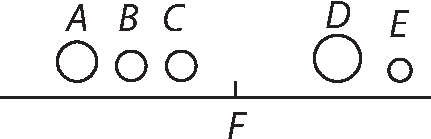
\includegraphics[width=0.3\textwidth]{%
gesamttex/edit_VIII,3/images/LH_38_212-215_d1_213r.pdf%
}} 
\vspace{0.5em}
\centerline{%
\lbrack\textit{Fig.~1}\rbrack%
}
% \newpage%
%\vspace{1.0em}
%
%
\newpage
\pstart
\noindent en des points
%
\edtext{ou que leur
%
\edtext{grosseur n'est pas compa\lbrack ra\rbrack ble à}{\lemma{grosseur}\Bfootnote{\textit{(1)} \textbar\ est \textit{streicht Hrsg.} \textbar\ incompable \textit{\lbrack\!!\rbrack} \textit{(2)} n'est pas \textbar\ compable \textit{ändert Hrsg.}\ \textbar\ à \textit{L}}} 
%
leur distance\lbrack,\rbrack}{\lemma{}\Bfootnote{ou que  \lbrack...\rbrack\ leur distance \textit{erg. L}}}
%
\edtext{autrement ils}{\lemma{autrement}\Bfootnote{\textit{(1)} ils ne sçavoient \textit{(2)} ils \textit{L}}} 
%
ne pourront arriver tous ensemble en \textit{F}. \lbrack+\rbrack\protect\vphantom() %
\pend
%
\vspace{1.2em} %%%%%%%%% Diagramm 2
\centerline{%
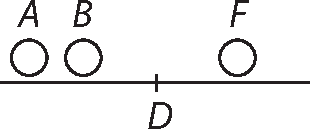
\includegraphics[width=0.225\textwidth]{%
gesamttex/edit_VIII,3/images/LH_38_212-215_d2_213r.pdf%
}} 
\vspace{0.5em}
\centerline{%
\lbrack\textit{Fig.~2}\rbrack%
}
% \newpage%
\vspace{0.8em}
%
%
\pstart
(\protect\vphantom)+ Examinons un peu la chose en trois corps, soit $AF\cdot A+BF\cdot B%
%
\edtext{= DF$. Le}{\lemma{\textit{DF}.}\Bfootnote{\textit{(1)}~Soit \textit{(2)}~Le \textit{L}}} 
%
centre de
%
\edtext{gravité sera \textit{F}. Et alors il est seur qu'ils}{\lemma{gravité}%
\Bfootnote{
\textit{(1)} \textit{G} \textit{(2)} sera \textit{G} \textit{(3)} sera \textit{F}. 
\textit{(a)} Mais alors 
\textit{(b)} Et alors il est seur
\textit{(aa)} que le centre \textit{(bb)}~qu'ils se choqueront avec equilibre. Mais il
\textit{(cc)} qu' \textbar\ alors \textit{streicht Hrsg.}\ \textbar\ ils \textit{L}}} 
%
se choqueront avec equilibre. 
%
\edtext{Cependant ils}{%
\lemma{Cependant \textbar\ mais}%
\Bfootnote{%
\textit{streicht Hrsg.}\ \textbar\ %
ils \textit{L}}} 
%
ne se choqueront pas en même temps, mais en differens temps selon leur grandeur, à moins qu'on ne les considere que comme des points.  \lbrack+\protect\vphantom()\rbrack
\pend
%
\pstart Ch.~15.
%
\edtext{Pour \textit{trouver le centre de masse\protect\index{Sachverzeichnis}{centre de masse}} (\lbrack+\rbrack\ c'est ainsi qu'il parle +) sur une même ligne
%
\edtext{droite, il}{\lemma{droite,}\Bfootnote{\textit{(1)} prenes un point \textit{G}, à souhait sur la droite multiplies chaque corps par sa \textit{(2)} il  \textit{ L}}} 
%
distingue deux cas, que le point pris à souhait soit
%
\edtext{hors des}{\lemma{hors}\Bfootnote{\textit{(1)} du point, ou \textit{(2)} des \textit{L}}} 
%
corps ou entre les corps. Au premier cas il adjoute seulement, au second il mele addition et soustraction, mais on peut dire generalement, que les progres de 
%
\edtext{ces corps vers}{\lemma{ces}\Bfootnote{corps \textit{(1)} d'un même sens \textit{(2)} vers \textit{L}}} 
%
ce point en même sens multipliés par les corps sont une somme la quelle 
%
\edtext{divisée par}{%
\lemma{divisée}%
\Bfootnote{%
\textit{(1)} par les corps %
\textit{(2)} par la somme donne %
\textit{(a)} la masse %
\textit{(b)} par %
\textit{L}%
}}
%
la
%
\edtext{somme donne le progres}{\lemma{somme}\Bfootnote{\textit{(1)} par les corps \textit{(2)} donne \textit{(a)} la masse \textit{(b)} le progres \textit{L}}} 
%
du centre
%
\edtext{vers ce point car lors qu'il}{\lemma{vers ce}\Bfootnote{\textit{(1)} corps \textit{(2)} point \textit{(a)} ce \textit{(b)} car \textit{(aa)} le \textit{(bb)} lors \textit{(aaa)} que \textit{(bbb)} qu'il \textit{L}}} 
%
y a un corps qui a besoin d'aller d'un autre sens, son progres dans le sens proposé est negatif.}{\lemma{Pour \textit{trouver} \lbrack...\rbrack\ est negatif}\Cfootnote{a.a.O., S.~49f.\cite{01500}}} \pend
%
\pstart Ch.~16.17.
%
\edtext{\textit{Loix du choc\protect\index{Sachverzeichnis}{loix du choc} direct des corps sans ressort}.}{\lemma{\textit{Loix du}  \lbrack...\rbrack\ \textit{sans ressort}}\Cfootnote{a.a.O., S.~50.\cite{01500}}} 
%
S'ils sont
%
\edtext{\lbrack en\rbrack}{\lemma{}\Bfootnote{en \textit{ erg. Hrsg.}}} 
%
equilibre ils reposent après le choc: si non ils iront tous ensemble après le choc, 
%
comme alloit le centre de
%
\edtext{masse. Les figures}{\lemma{}\Bfootnote{masse. \textbar\ (+ Il ne considere point le cas des corps qui ont moitié ressort, et moitié point +) \textit{gestr.} \textbar\ Les figures \textit{L}}} 
%
sont changés, comme si ces corps rencontroient
%
\edtext{\textit{un corps infiniment dur avec}}{\lemma{\textit{un corps infiniment dur avec}}\Cfootnote{a.a.O., S.~58.\cite{01500}}} cette force qu'il a.
\pend
\newpage
%
\pstart
%
\hspace{1mm}\hspace{-1mm}% Trick, weil \edlabel nicht zu \par-Beginn sein darf
%
\edlabel{38_212-215_8a}%
\edtext{}{%
{\xxref%
{38_212-215_8a}{38_212-215_8b}}%
\lemma{Ch.~18. \lbrack...\rbrack\ \textit{parfait}}%
\Cfootnote{%
a.a.O., S.~58.\cite{01500}}}%
\edtext{Ch.~18. Dans}{\lemma{Ch.~18.}\Bfootnote{\textit{(1)} Quand deux c \textit{(2)} Dans \textit{L}}} 
%
le choc \textit{des corps à ressort parfait}\edlabel{38_212-215_8b}
%
s'ils se choquent avec equilibre chacun doit retourner avec sa vistesse premiere, d'où il tire tout le reste avec l'aide du plan auxiliaire. C'est à dire s'ils concourent sans opposition, et si
%
%
\edlabel{38_212-215_9a}%
\edtext{}{%
{\xxref%
{38_212-215_9a}{38_212-215_9b}}%
\lemma{après \lbrack...\rbrack\ \textit{opposition}}%
\Cfootnote{%
a.a.O., S.~61.\cite{01500}}}%
\edtext{après \lbrack le\rbrack\ choc il}{%
\lemma{après}%
\Bfootnote{%
\textbar\ le \textit{erg. Hrsg.}\ \textbar\ choc %
\textit{(1)} il y a %
\textit{(2)} il %
\textit{L}%
}}
%
\textit{n'y a point d'opposition}\edlabel{38_212-215_9b}
%
non plus; il demeure la même force selon
%
\edtext{l'auteur; et la somme}{\lemma{l'auteur}\Bfootnote{\textit{(1)} . Mais s'ils se separent avec opposition \textit{(2)} ; et la somme \textit{L}}} 
%
avant le choc est egale a la somme après le choc. Mais s'ils se separent avec 
%
\edtext{opposition alors la somme des mouvemens est augmentée.}{\lemma{opposition}\Bfootnote{\textit{(1)}~alors la somme avant le choc est égale \textit{(a)} ave \textit{(b)} à la somme après le choc. Quand il y a la somme \textit{(2)} alors \lbrack...\rbrack\ augmentée. \textit{L}}} 
%
De même s'ils concourent avec
%
\edtext{opposition et vont}{\lemma{opposition}\Bfootnote{\textit{(1)} et se separent avec opposition \textit{(2)} et vont \textit{L}}} 
%
après du même
%
\edtext{costé, la somme des mouvemens est diminuée.}{\lemma{costé,}\Bfootnote{\textit{(1)}~la force est diminuée \textit{(2)} la somme des mouvemens est diminuée. \textit{L}}}
%%
\pend
%
\pstart
%
\edtext{\textit{Regle generale} (en prenant la force pour la quantité de mouvement)\;\lbrack\!\!:\rbrack\
%
\textit{en prenant deux differens temps egaux}\lbrack,\rbrack\ \textit{l'un devant l'autre après le choc, si l'un 
%
contient de l'opposition et que l'autre n'en ait point, celuy qui en contient aura tousjours la plus grande 
%
quantité\protect\index{Sachverzeichnis}{quantité de force} de force}}{\lemma{}\Cfootnote{\hspace{-2.8mm}\textit{Regle generale}  \lbrack...\rbrack\ \textit{de force}:\hspace{1mm} a.a.O., S.~64 mit Auslassung.\cite{01500}}} 
%
absolue\protect\index{Sachverzeichnis}{force absolue} mais la relative\protect\index{Sachverzeichnis}{force relative} est tousjours la même. 
%
\lbrack213~v\textsuperscript{o}\rbrack
\pend
%
%
\vspace{1.5em} %%%%%%%%% Diagramm 3
\centerline{%
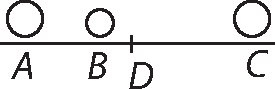
\includegraphics[width=0.2\textwidth]{%
gesamttex/edit_VIII,3/images/LH_38_212-215_d3_213v.pdf%
}} 
\vspace{0.5em}
\centerline{%
\lbrack\textit{Fig.~3}\rbrack%
}
% \newpage%
\vspace{1.0em}
%
%
\pstart  
Ch.~19. 
%
\edlabel{38_212-215_213v1}%
\edtext{}{{\xxref{38_212-215_213v1}{38_212-215_213v2}}\lemma{\textit{Loy generale} \lbrack...\rbrack\ \textit{soyent egaux}}\Cfootnote{a.a.O., S.~65f.\ mit Auslassungen.\cite{01500}}}%
%
\textit{Loy generale du ressort\protect\index{Sachverzeichnis}{ressort} parfait entre tant de corps que ce soit}: \textit{Si trois corps parexemple \textit{A}, \textit{B}, \textit{C}, doivent se rencontrer 
%
\edtext{en même temps en \textit{D},}{%
\lemma{}%
\Bfootnote{%
en même temps en \textit{D} %
\textit{erg.\ L}%
}}
%
je divise l'instant de leur choc en plusieurs parties; dans la premiere \textit{B} et \textit{C} se choquant %
%
en \textit{D}} \textit{suivent les loix de deux corps à ressort qui se choquent en sens contraire. 
%
Dans la seconde \textit{A} rencontre \textit{B} avec toute sa force\protect\index{Sachverzeichnis}{force}, et celle que \textit{B} a contractée par le}
%
\edtext{\textit{choc au}}{\lemma{\textit{choc}}\Bfootnote{\textit{(1)} en \textit{(2)} \textit{au} \textit{L}}} 
%
\textit{quel cas ils suivent encor les loix de deux corps à ressort. 
%
Dans la 3\textsuperscript{me} partie}\lbrack,\rbrack\ \textit{supposé que \textit{B} doive encor rencontrer \textit{C} 
%
avec la vistesse que \textit{B} a contractée dans le second choc et celle que \textit{C} a contractée dans le premier}\lbrack,\rbrack\ 
%
\textit{ils suivront encor les mêmes loix precedentes; 
%
Enfin dans la 4\textsuperscript{me} partie de l'instant du choc, supposé que \textit{A} doive une seconde fois rencontrer \textit{B}, ils agiront l'un contre l'autre}\lbrack,\rbrack\
%
\textit{sçavoir \textit{A} avec la force qu'il a contractée par le second choc, et \textit{B} avec celle qu'il a acquise
%
par le 3\textsuperscript{me}, et ainsi de suite, jusqu'à ce que ces trois corps ne doivent plus se rencontrer}\lbrack,\rbrack\ \textit{ce qui se reconnoistra tousjours en calculant}
%
\edtext{\textit{leur}\lbrack \textit{s}\rbrack}{\lemma{}\Bfootnote{leur \textit{ L ändert Hrsg. nach Vorlage}}} 
%
\textit{vistesses suivant les loix des deux corps, quelque nombre de corps qu'il y ait, et en quelque sens qu'}il \textit{se} rencontre \textit{sur la droite \textit{AB}.}%
\pend
%
\pstart
%
\textit{Il suit de} cela \textit{que si l'on a sur une ligne droite plusieurs corps à ressort qui soyent egaux}%
\edlabel{38_212-215_213v2}
%
\edtext{et}{\lemma{\textit{egaux}}\Bfootnote{\textit{(1)} \textbar\ il ne se \textit{ streicht Hrsg.} \textbar\ mettra jamais après le choc en mouvement qu' \textit{(2)} et \textit{L}}} 
%
qu'un certain nombre en choque d'autres en repos, il ne se mettra
%
\edtext{\textit{jamais après le choc en mouvement qu'autant qu'il y en avoit auparavant.}}{\lemma{\textit{jamais après}  \lbrack...\rbrack\ \textit{avoit auparavant}}\Cfootnote{a.a.O., S. 68.\cite{01500}}} \pend
%
\pstart Ch.~20. 
%
\edtext{\textit{Quand deux corps de pareille matiere
et figure se choqueront il arrivera la même chose à l'egard du centre commun de masse, 
et à l'egard de leur force ou mouvement commun\protect\index{Sachverzeichnis}{mouvement commun}, 
que si ces corps avoient un ressort parfait ou n'en avoient point du tout. 
Mais lors que leur matieres sont heterogenes}\lbrack,\rbrack\ \textit{les proprietes cy dessus n'auront plus de lieu},}{%
\lemma{\textit{Quand deux}\lbrack...\rbrack\ \textit{lieu}}%
\Cfootnote{%
a.a.O., S. 72 mit Auslassung.\cite{01500}
%
}}
%
car ce n'est plus le centre commun de masse\protect\index{Sachverzeichnis}{centre de masse}
%
(+ mais il restera tousjours le centre commun de pesanteur qui demeurera en repos comme auparavant +).% 
\pend 
%
%
%
\pstart
%
\edtext{% C-Fn Stellenangabe
\textit{Les deux loix} generales
%
que l'auteur met pour toute sorte de ressorts parfaits ou
%
\edtext{imparfait\lbrack s\rbrack}{\lemma{}\Bfootnote{imparfaites \textit{L ändert Hrsg.}}} 
%
\edtext{\lbrack \textit{se}\rbrack}{%
\lemma{}%
\Bfootnote{%
se %
\textit{erg.\ Hrsg.\ nach Vorlage}%
}}
%
\textit{reduisent à cette loy generale, que j'ay demonstrée} (dit il) 
%
\edtext{\textit{dans le Journal des Sçavans 4\textsuperscript{me} May 1699.}}{%
\lemma{\textit{dans} \lbrack...\rbrack\ \textit{1699}}%
\Cfootnote{%
\protect\index{Namensregister}{\textso{Parent}, Antoine 1666\textendash1716}\textsc{A.~Parent}, \cite{02029}\glqq Loy universelle pour quelque multitude de corps que ce soit\grqq, 
\cite{00157}\textit{JS} (Pariser Ausgabe), 4.~Mai 1699, S.~197\textendash200.}}
%
\textit{Dans tous les chocs \textso{sur une ligne droite}, les corps conservent la loy de leur equilibre à l'egard du point \textit{c} de l'immensité qui se meut de la même vistesse après le choc dont alloit} avant \textit{le choc leur}
%
\edtext{\textit{centre commun}}{\lemma{\textit{centre}}\Bfootnote{\textit{(1)} dont allo \textit{(2)} \textit{commun} \textit{L}}} 
%
\textit{de}}{%	% C-Fn Stellenangabe
\lemma{\textit{Les deux}  \lbrack...\rbrack\ \textit{commun de}}\Cfootnote{a.a.O., S.~72f. mit Auslassung.\cite{01500}}}
%
gravité. %
\pend
%
\vspace{1.5em} %%%%%%%%% Diagramm 4
\centerline{%
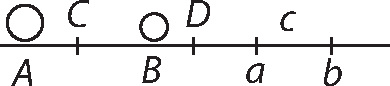
\includegraphics[width=0.3\textwidth]{%
gesamttex/edit_VIII,3/images/LH_38_212-215_d4_213v.pdf%
}} 
\vspace{0.5em}
\centerline{%
\lbrack\textit{Fig.~4}\rbrack%
}
% \newpage%
\vspace{1.0em}
%
\pstart
\edtext{Corps}{%
\lemma{\hspace{1.6mm}%
\lbrack\textit{Fig.~4}\rbrack%
}\killnumber%
\Cfootnote{%
tlw.\ Übernahme der Vorlage: \textsc{Parent}, \textit{Élémens}, Pl.~2, Fig.~29.\cite{01500}%
}}
%
\textit{A}, \textit{B}, leur centre\protect\index{Sachverzeichnis}{centre commun} commun
%
\edtext{\textit{C}, le}{\lemma{\textit{C},}\Bfootnote{\textit{(1)} leur \textit{(2)} le \textit{L}}} 
%
lieu du choc \textit{D}; le progres du centre de gravité\protect\index{Sachverzeichnis}{centre de gravité} 
%
\edtext{avant le choc, \textit{CD},}{%
\lemma{avant le choc,}%
\Bfootnote{%
\textit{(1)} le progres %
\textit{(2)} \textit{CD}, %
\textit{L}%
}}
%
le progres du point \textit{c} après le choc \textit{cD}; 
%
le progres du corps \textit{A}, \textit{Aa}, le progres du corps \textit{B}, \textit{Bb}. 
%
Les \textit{AC} estant \textit{u}, $ac\;\displaystyle\frac{g}{u}$,\rule[-2mm]{0pt}{8mm} 
%
si le ressort n'est pas parfait; et \textit{BC} estant \textit{v}, \textit{bc} sera $\displaystyle\frac{g}{v}$.\rule[-2mm]{0pt}{8mm} 
%
(\protect\vphantom)+ Je m'estonne de cela, il falloit \rule[-4mm]{0pt}{10mm}$\displaystyle\frac{u}{g}$, ou $\displaystyle\frac{v}{g}$\rule[-4mm]{0pt}{10mm}, car ainsi
%
\edtext{le cas}{\lemma{le}\Bfootnote{\textit{(1)} choc du ress \textit{(2)} cas \textit{L}}} 
%
du ressort imparfait\protect\index{Sachverzeichnis}{ressort imparfait} evanouiroit dans celuy du ressort parfait.
%
\edtext{Je trouve par le calcul qu'il l'a entendu ainsi.}{\lemma{}\Bfootnote{Je trouve \lbrack...\rbrack\ ainsi \textit{erg. L}}} 
%
+\protect\vphantom()%
\pend
%
\pstart
%
%
%
\edtext{\edtext{%	A-Fn zur Rechnung
%
\textit{CD} ou $cD=A\cdot AD\;\pleibdashv B\cdot BD,:,A+B$. 
%
$AC=AD-CD=B\cdot AD \;\pleibvdash B\cdot BD,:,A+B$ 
%
et $BC=CD\;\pleibvdash BD=A\cdot AD\;\pleibvdash A\cdot BD,:,A+B$. 
%
Donc $ac= (AD\;\pleibvdash BD) Bu: (a+b)g$ et $bc=(AD\;\pleibvdash BD)AV:(A+B)g$.%
%
}{\lemma{}\Afootnote{%
\foreignlanguage{ngerman}{\textit{Am Rand, durch ein Verweiszeichen auf die Rechnung bezogen}:}
Je reduiray le calcul de l'auteur different pour le cas\textsuperscript{\lbrack a\rbrack} sans opposition, ou avec opposition à ce calcul general, et $\pleibdashv$ signifiera $+$ dans le premier cas, et $-$ dans le second.
\newline\vspace{-0.5em}\newline%Marginalienapparat:
{\footnotesize \textsuperscript{\lbrack a\rbrack} cas \textit{(1)} de l'opposition \textit{(2)} sans \textit{ L}}%
}}}{%
\lemma{\textit{CD} \lbrack...\rbrack\ $(A+B)g$}%
\Cfootnote{%
Vgl. a.a.O., S.~69.\cite{01500}\hspace{-2mm}%
}}
%
\pend
%
\pstart%%%%%%%%%%%%%%%%%%%%
Hinc tandem 
%
\edlabel{38_212-215_10a}%
\edtext{}{%
{\xxref%
{38_212-215_10a}{38_212-215_10b}}%
\lemma{$Da$ \lbrack...\rbrack\ $(a+b)g$}%
\Cfootnote{%
Vgl. a.a.O., S.~70.\cite{01500}\hspace{-2mm}}}%
$Da=Dc-ca=(A\cdot AD\;\pleibdashv B\cdot BD)g-(AD\;\pleibvdash BD)Bu,:(a+b)g$%
\pend
%
\pstart
et 
\phantom{iii tandem} $Db=Dc+cb=(A\cdot AD\;\pleibdashv B\cdot BD)g+(AD\;\pleibvdash BD)AV,:(a+b)g$.%
\edlabel{38_212-215_10b} 
\pend
%
\pstart (+ Toutes ces choses \edtext{not\lbrack é\rbrack es}{\lemma{}\Bfootnote{notes \textit{L ändert Hrsg.}}}
sont assez connües. +) 
%
\edtext{Or \textit{il faut bien remarquer} (adjoute l'auteur\lbrack)\rbrack\ \textit{que si \textit{ac} est encor à \textit{cb}, comme \textit{AC} à \textit{CB}, c'est à dire si les ressorts de ces corps sont semblables}\lbrack,\rbrack\ \textit{le point \textit{c} sera} le \textit{centre commun de} leur \textit{masse}; car c'est tousjours comme \textit{B} à \textit{A} 
%
\edtext{ou \textit{b} à \textit{a}; ainsi \textit{le centre de masse} ne change point \textit{de vistesse par le choc}.}{%
\lemma{}%
\Bfootnote{%
ou \textit{b} à \textit{a} %
\textit{erg.\ L}%
}}}{%
\lemma{\textit{il f\hspace{0.5mm}}}%
\Cfootnote{%
\hspace{-3.1mm}\textit{aut} \lbrack...\rbrack\ \textit{choc}:\hspace{1mm} a.a.O., S.~70f. mit Auslassungen.\cite{01500}
}}
%
%
\edtext{\textit{Mais lorsque} \edtext{\textit{leur}\lbrack \textit{s}\rbrack}{\lemma{}\Bfootnote{leur \textit{L ändert Hrsg.}}} 
%
\textit{matieres sont heterogenes,}
\textit{c ne sera plus} le \textit{centre commun de} leur \textit{masse}.}{%
\lemma{\textit{Mais} \lbrack...\rbrack\ \textit{masse}}%
\Cfootnote{%
a.a.O., S.~72 mit Auslassungen.\cite{01500}
%
}}
%
(+ Pourquoy? Est ce qu'ils se transforment\,\lbrack\!?\rbrack\ Mais alors aussi il ne faut considerer ces corps seuls, mais leur parties insensibles. Et si on considere les touts seulement, il faut considerer les corps comme des points. \lbrack+\rbrack) \pend
%
\pstart
%
\edtext{Ch.~21. Quand}{\lemma{Ch.~21.}\Bfootnote{\textit{(1)} Quoyque les parties \textit{(2)} Quand \textit{L}}} 
%
on considere l'epaisseur des
%
\edtext{corps, il}{\lemma{corps,}\Bfootnote{\textit{(1)} les point \textit{\lbrack\!!\rbrack} de rencontre ou d'attou \textit{(2)} il \textit{(3)} il \textit{L}}} 
%
n'en vient aucune
%
\edtext{incommodite. (\protect\vphantom)+ L'auteur}{\lemma{incommodite}\Bfootnote{\textit{(1)} , car on peut prendre au lieu des corps, les points où ils se touchent (\protect\vphantom)+ l'auteur ne \textit{(2)} . (\protect\vphantom)+ L'auteur \textit{L}}} 
%
ne l'explique pas bien, mais on peut prendre le tout comme si les corps qui se rencontrent
%
\edtext{estoient concentrés}{\lemma{estoient}\Bfootnote{\textit{(1)} reunis dans les points \textit{(2)} concentrés \textit{L}}} 
%
dans les points où ils se touchent. Il faut examiner
%
\edtext{si dans}{\lemma{si}\Bfootnote{\textit{(1)} après le point de \textit{(2)} dans \textit{L}}} 
%
le concours de deux corps qui se rencontrent avec equilibre, les deux points de 
%
\edtext{rencontre se}{%
\lemma{rencontre}%
\Bfootnote{%
\textit{(1)} se cedent %
\textit{(2)} se %
\textit{L}%
}}
%
resistent egalement, quoyque les corps soyent inegaux. 
%
On peut s'imaginer comme si les corps estoient composés de parties
%
\edtext{rigides qui font la masse, entrelassés}{\lemma{rigides}\Bfootnote{\textit{(1)} , composées 
\textit{(2)} \textbar\ entrelacés \textit{streicht Hrsg.}\ \textbar\ de parties elastiques
\textit{(3)} \textbar\ qui font la masse \textit{erg.}\ \textbar\ , entrelassés \textit{L}}} 
%
de ressorts 
%
\edtext{%	A-Fn
dont on ne considere point la masse; en ce cas, imaginant que les parties 
%
rigides sont tousjours egales, et se rencontrent directement, 
%
on en deduira le tout. On pourra aussi s'imaginer, les concours obliques, et deduire
%
\edtext{leur\lbrack s\rbrack}{\lemma{}\Bfootnote{leur \textit{ L ändert Hrsg.}}} loix, quoyque les corps soyent composés de globes egaux. +\protect\vphantom()%
}{%
\lemma{}%
\Afootnote{%
\foreignlanguage{ngerman}{\textit{Am Rand:} NB}}}%
%
\pend
%
\pstart 
%
Ch.
%
\edtext{\lbrack22.\rbrack}{\lemma{}\Bfootnote{21. \textit{L ändert Hrsg.}}} 
%
L'auteur
%
\edtext{rapporte les}{\lemma{rapporte}\Bfootnote{\textit{(1)} les centres de masse \textit{(2)} les \textit{ L}}} 
%
%
\edtext{\textit{proprietes du centre de masse} (de pesanteur) \textit{entre les corps qui sont situés hors une même ligne droite}.}{%
\lemma{\textit{proprietes} \lbrack...\rbrack\ \textit{droite}}%
\Cfootnote{%
a.a.O., S.~75.\cite{01500}
%
}}
% 
Mais ces proprietes sont
%
\edtext{connu\lbrack e\rbrack s}{\lemma{}\Bfootnote{connus \textit{L ändert Hrsg.}}}.
\pend
%
%
\vspace{1.5em}		%Fig. 5
\centerline{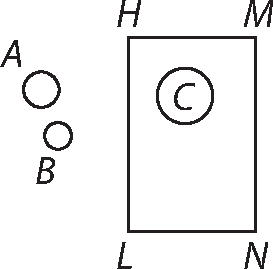
\includegraphics[width=0.2\textwidth]{gesamttex/edit_VIII,3/images/LH_38_212-215_d5_213v.pdf}}
\vspace{0.5em}
\centerline{\lbrack\textit{Fig.~5}\rbrack}
\vspace{1.0em}
%
\pstart
%
\edtext{Ch.~\lbrack23.\rbrack}{%
\lemma{}%
\Bfootnote{%
22. \textit{L ändert Hrsg.}}
\lemma{\hspace*{1,6mm}%
\lbrack\textit{Fig.~5}\rbrack%
}\killnumber%
\Cfootnote{%
tlw.\ Übernahme der Vorlage: a.a.O., Pl.~2, Fig.~33.\cite{01500}%
}}
%
\edtext{Il \textit{suppose que les corps A et B},}{%
\lemma{\textit{suppose} \lbrack...\rbrack\ \textit{B}}%
\Cfootnote{%
a.a.O., S.~78.\cite{01500}
%
}}
%
\edtext{\textit{C}, allant}{\lemma{\textit{C},}\Bfootnote{\textit{(1)} rencontrent \textit{(2)} allant \textit{L}}} 
%
en lignes paralleles entre \mbox{elles} choquent en même temps le solide
%
\edtext{inebranslable}{\lemma{}\Bfootnote{inebranslable \textit{erg. L}}} 
%
\textit{HL} et que la quantité de mouvement de \textit{C}, soit egale à celles d'\textit{A} et \textit{B}. 
%
Il y aura encor equilibre. 
%
Et de même si sans le corps inebranslable, ils se choquoient immediatement 
%
(+ mais alors \textit{A} et \textit{C} reflechiront tout autrement, que si \textit{HL} estoit interposé +). 
%
Donc il en sera de même, si on adjoute de \makebox[1.0\textwidth][s]{plus 
%
\edtext{\lbrack un\rbrack}{%
\lemma{}%
\Bfootnote{%
un %
\textit{erg.\ Hrsg.}%
}}
%
certain mouvement du plan sur le quel ils sont. 
%
Il raisonne de même s'il y avoit}
\pend
\newpage
\pstart
\noindent plusieurs tels chocs à la fois sur un même solide \textit{HLNM}. 
%
Car on pourra \edtext{tousjours les reduire}{%
\lemma{tousjours}%
\Bfootnote{les %
\textit{(1)}~retirer %
\textit{(2)} reduire %
\textit{L}%
}}
%
%
\edtext{à \edtext{\textit{l'equilibre, en retirant}}{
\lemma{l'equilibre,}
\Bfootnote{\textit{(1)} en adjoutant un mouvement du coste du plus fort \textit{(2)} en retirant \textit{ L}}} 
\textit{le lieu où sont ces corps du sens contraire aux plus forts}.}{%
\lemma{\textit{l'equilibre} \lbrack...\rbrack\ \textit{forts}}%
\Cfootnote{%
a.a.O., chap.~XXIV, S.~80f.\cite{01500}
%
}}
%
(+ L'auteur reduit le cas proposé à l'equilibre, en donnant au lieu un sens contraire un mouvement du centre de gravité. +) 
%
(+ L'auteur parle comme si par le moyen du choc que font les corps sur un plan rigide entre eux, il expliquoit le choc des corps sur des paralleles, mais cela n'est point, car la reflexion se fait tout autrement. +) 
%
(\protect\vphantom)+ Comme il n'avoit
%
\edtext{pas un principe}{\lemma{}\Bfootnote{pas un \textbar\ bon \textit{gestr.} \textbar\ principe \textit{L}}} 
%
bien seur dans sa division des instans\lbrack,\rbrack\ il n'a pas osé l'appliquer à des concours des corps 
%
hors d'une même ligne droite. C'est qu'il ne sçavoit pas 
%
\edtext{mon principe de la loy des continuités.\protect\index{Sachverzeichnis}{loi des continuités}}{%
\lemma{mon \lbrack...\rbrack\ continuités}%
\Cfootnote{%
Siehe \protect\index{Namensregister}{\textso{Leibniz} (Leibnitius, GGL), Gottfried Wilhelm 1646\textendash1716}\textsc{G.\,W.~Leibniz}, 
\cite{02054}\textit{Extrait d'une lettre de M.~L.\ sur un principe général}, 
\cite{02002}\textit{Nouvelles de la République des lettres}, Juli 1687, S.~744\textendash753, sowie \textsc{Ders.}, \cite{02055}\textit{Principium quoddam generale}, \textit{LSB} VI, 4 N.~371, S.~2031\textendash2039.}}
%
+\protect\vphantom() \lbrack214~r\textsuperscript{o}\rbrack\
\pend
%
%214r
%
\vspace{1.0em}
\pstart
\centering
\protect\index{Namensregister}{\textso{Parent}, Antoine 1666\textendash1716}Parent 
\cite{01500}\textit{Elemens de Mecanique} seconde partie
\pend %Keine Leerzeile
%
\pstart\noindent Ch.~1. Du choc des corps mûs à l'entour \textit{d'un point fixe, sur une même circomference}\edtext{}{\lemma{\textit{d'un point}  \lbrack...\rbrack\ \textit{circomference}}\Cfootnote{\textsc{Parent}, \textit{Élémens}, S.~83.\cite{01500}}}. C'est tout comme s'ils estoient sur une même ligne droite. 
%
(\protect\vphantom)+ Il ne le prouve point. Mais c'est qu'on peut reduire ces chocs à des chocs 
%
droits\protect\index{Sachverzeichnis}{choc droit} differens des circulaires aussi peu que l'on voudra. 
%
Les corps aussi
%
\edtext{estant incomparablement}{\lemma{estant}\Bfootnote{\textit{(1)} petits \textit{(2)} d \textit{(3)} inco \textit{(4)} i \textit{(5)} incomparablement \textit{L}}} 
%
petits à comparaison des rayons, paroissent choquer sur une même droite aux 
%
spectateurs\protect\index{Sachverzeichnis}{spectateur} qui seroient sur ces corps.
\lbrack+\protect\vphantom()\rbrack\
\pend 
%
%
\pstart Ch.~2. L'auteur le trouve encor comme des chocs droits en se servant d'un rayon auxiliaire
%
\edtext{\textit{pour reduire ce choc à}}{\lemma{\textit{pour reduire}  \lbrack...\rbrack\ \textit{l'equilibre}}\Cfootnote{a.a.O., S. 84.\cite{01500}}}
%
\edtext{\textit{l'equilibre\edlabel{38_212-215_214r1}}.}{{\xxref{38_212-215_214r1}{38_212-215_214r2}}\lemma{\textit{l'equilibre}.}\Bfootnote{%
\textit{(1)} Si on a 
\textit{(2)} Supposant comme un centre de masses à l'imitation des \textit{(a)} droit \textit{(b)} chocs droits, c'est à dire que les arcs 
\textit{(3)} Quand même ces corps n'iroient pas sur la même circomference mais sur des arcs concentriques. Et il s'imagine encor à leur imitations un centre de masse, c'est à dire en sorte que les quantites des mouvemens circulaires soyent
\textit{(4)} \textbar\ Si les corps \textit{streicht Hrsg.}\ \textbar\ %
\textit{(a)} alloit 
\textit{(b)} \textbar\ alloient \textit{streicht Hrsg.}\ \textbar\ choquer le rayon qui passe par ce centre 
\textit{(5)} Ch.~3. \textit{L}}} 
%
\pend 
\newpage
%
%\vspace{1.5em}
\centerline{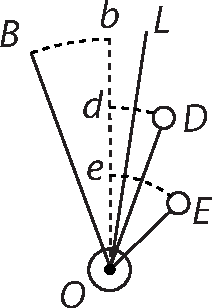
\includegraphics[width=0.16\textwidth]{gesamttex/edit_VIII,3/images/LH_38_212-215_d6_214r.pdf}}
\vspace{0.5em}
\centerline{\lbrack\textit{Fig.~6}\rbrack} 
\vspace{1.5em}
%
\pstart
\edtext{Ch.~3.\edlabel{38_212-215_214r2}}{%
\lemma{\hspace*{1,6mm}%
\lbrack\textit{Fig.~6}\rbrack%
}\killnumber%
\Cfootnote{%
tlw.\ Übernahme der Vorlage: a.a.O., Pl.~3, Fig.~36.%
}}
%
Quand ces corps ne vont pas sur la même circomference, mais sur des circonferences 
%
eccentriques\protect\index{Sachverzeichnis}{circonference eccentrique}, il ne se sert plus des arcs 
%
mais des secteurs. Par exemple supposant que les corps \textit{B}, \textit{D}, \textit{E}, soyent attachés à
%
 des rayons solides\protect\index{Sachverzeichnis}{rayon solide} \textit{OB}, \textit{OD},
%
 \textit{OE}, mobiles dans un même
%
\edtext{plan, à}{\lemma{plan,}\Bfootnote{\textit{(1)} sur \textit{(2)} à \textit{L}}} 
%
l'entour du centre \textit{O}. Et qu'ils aillent se choquer par le moyen de leur rayons, 
%
au rayon \textit{Oebd}; il dit qu'à fin qu'ils fassent equilibre
%
il faut que la somme des secteurs de mouvement, 
%
\edtext{multipliés chacun}{\lemma{multipliés}\Bfootnote{\textit{(1)} par \textit{(2)} chacun \textit{L}}} 
%
par son mobile, soyent egales de part et d'autre. Ainsi $BOb.B$ sera egal icy à $DOd.D+EOe.E$.
%
(\protect\vphantom)+ Il n'en rend aucune raison et il semble 
%
\edtext{fort}{%
\lemma{}%
\Bfootnote{%
fort %
\textit{erg.\ L}%
}}
%
qu'il faudroit plustost prendre les
%
\edtext{arcs, et faire}{\lemma{arcs,}\Bfootnote{\textit{(1)}~\textbar\ et \textit{streicht Hrsg.}\ \textbar\ dire \textit{(2)} et faire \textit{L}}} 
%
$Bb.B=Dd.D+Ee.E$. Mais la veritable raison est, que le corps \textit{B}, fait plus non seulement 
%
\edtext{s'il choque}{%
\lemma{s'il}%
\Bfootnote{%
\textit{(1)} vient avec un ar %
\textit{(2)} choque %
\textit{L}%
}}
%
dans un arc plus grand, comme \textit{Bb}, mais aussi parce
%
\edtext{qu'il choque dans un}{\lemma{qu'il}\Bfootnote{\textit{(1)} vient avec un ar \textit{(2)} choque dans un \textit{L}}} 
%
endroit plus eloigné du centre \textit{O}, comme \textit{b}. Pour proceder par ordre, il auroit
%
\edtext{fa\lbrack ll\rbrack u}{\lemma{}\Bfootnote{falu \textit{L ändert Hrsg.}}}
%
\edtext{distinguer les centres des arcs \textit{Bb}, et le centre}{\lemma{distinguer}\Bfootnote{\textit{(1)} les ar \textit{(2)} les centres des arcs \textit{Bb}, et \textit{(a)} les centres \textit{(b)} le centre \textit{L}}}
%
%
du rayon dans lequel se fait le choc, qui pourroient estre differens.
%
\edtext{Même il se}{\lemma{Même}\Bfootnote{\textit{(1)} les mo \textit{(2)} il se \textit{L}}} 
%
pourroit que le mouvement de \textit{B} fut à l'entour d'un centre, et celuy du moment 
%
\edtext{\textit{d}, à l'entour d'un autre.}{\lemma{\textit{d},}\Bfootnote{à l'entour d'un \textit{(1)} autre. Item \textit{(a)} que le choc se fit \textit{(b)} soit que le \textit{(c)} qu'il survint \textit{(d)} le rayon dans l' \textit{(2)} autre. \textit{L}}} 
%
Item qu'il se melât un corps qui allât choquer
%
en même temps par un choc droit\protect\index{Sachverzeichnis}{choc droit}. 
%
\edtext{Ainsi la vraye regle}{\lemma{}\Afootnote{\foreignlanguage{ngerman}{\textit{Am Rand}:} NB\vspace{-4mm}}} 
%
est de
%
\edtext{multiplier la vistesse}{\lemma{multiplier}\Bfootnote{\textit{(1)} le choc \textit{(2)} la vistesse \textit{L}}} 
%
du choc, par la distance du \makebox[1.0\textwidth][s]{centre du choque, ou la distance du corps qui choque par la distance du corps 
%
choqué. On}
\pend
\newpage
\pstart
\noindent voit aussi par là quand on compare des secteurs de differens cercles ce n'est plus comme la 
%
comparaison des angles. \lbrack+\protect\vphantom()\rbrack\
%
Après cela posé,
%
\edtext{l'auteur appelle}{\lemma{l'auteur}\Bfootnote{\textit{(1)} s'imagine aussi un point \textit{(2)} appelle \textit{L}}}
%
ce rayon
%
\edtext{d'equilibre, sur}{\lemma{d'equilibre,}\Bfootnote{\textit{(1)} Rayon \textit{(2)} sur \textit{L}}} 
%
le quel le choc se fait avec equilibre;
%
\edtext{\textit{\textso{Rayon de}
%
\edlabel{38_212-215_2a}%
\edtext{}{% 
{\xxref%
{38_212-215_2a}{38_212-215_2b}}%
\lemma{\textso{Masse}.}\Bfootnote{\textit{(1)} Si plusieurs corps \textit{(2)} Si plusieurs corps estoient attachés \textit{(3)} Si ces corps \textit{(a)} n'estoient pas à l'equilibre \textit{(b)} \textit{B}, \textit{L}}}%
\textso{Masse}}.}{\lemma{\textit{\textso{Rayon de Masse}}}\Cfootnote{a.a.O., S.~88.\hspace{20mm}}}
% 
Si ces corps \textit{B},%
\edlabel{38_212-215_2b}
%
\textit{D}, \textit{E} n'estoient pas à l'equilibre, le rayon de masse avanceroit, et si on y attachoit les corps \textit{B}, \textit{D}, 
%
\edtext{\textit{E}, en}{%
\lemma{\textit{E},}%
\Bfootnote{%
\textit{(1)} pour %
\textit{(2)} en %
\textit{L}%
}}
%
\textit{b}, \textit{d}, \textit{e}, 
%
pour aller avec ce rayon, ils feroient autant sur le rayon 
\edtext{\textit{OL}}{\lemma{}\Bfootnote{\textit{OL} \textit{erg. L}}} 
%
qu'ils rencontreroient, que feroient ces corps venant tous ensemble mais
\edtext{à part et sur leur\lbrack s\rbrack\ propres}{\lemma{{à} part}\Bfootnote{\textit{(1)} rencontrer ce rayon \textit{(2)} et sur \textbar\ leur \textit{ändert Hrsg.} \textbar\ propres \textit{L}}} 
%
rayons \textit{OB}, \textit{OD}, \textit{OE}, rencontrer ce Rayon \textit{OL}.
%
(+ Il falloit plustost appeller Rayon d'equivalence. +) 
%
Après l'auteur determine les choses à l'imitation des chocs droits.
%
(+ Il auroit encor pû appliquer les chocs droits à un rayon. \lbrack+)\rbrack
\pend 
%
\pstart
%
%
%
\edtext{
\edtext{Ch.~7.}{\lemma{ch.}\Bfootnote{\textit{(1)} 8. \textit{(2)} 9. \textit{(3)} 7. \textit{L}}} 
%
Il fait choquer directement les corps \textit{B}, \textit{D}, \textit{E}, contre le rayon \textit{Oedb}, mais il dit, qu'on peut imaginer que sur la fin ces
%
\edtext{lignes droites}{\lemma{lignes}\Bfootnote{\textit{(1)}~directes \textit{(2)} droites \textit{L}}} 
%
des chocs directs soyent des portions de
%
cercle infiniment 
%
\edtext{petites\lbrack,\rbrack\ mais}{%
\lemma{petites}%
\Bfootnote{%
\textit{(1)} en cherchant un point \textit{O} %
\textit{(2)} mais
\textit{L}%
}}
%
cela suppose que les vistesses soyent comme ces distances et alors 
%
tout se fait comme dans les chocs circulaires\protect\index{Sachverzeichnis}{choc circulaire} susdits. 
%
\edtext{Mais ce}{%
\lemma{Mais}%
\Bfootnote{%
\textit{(1)} ce ne s %
\textit{(2)} ce %
\textit{L}%
}}
%
n'est qu'un cas fort singulier. 
}{%
\lemma{Il fait \lbrack...\rbrack\ singulier}%
\Cfootnote{%
a.a.O., S.~100\textendash102.\cite{01500}%
}}
%
\pend 
%
\pstart C.~8. Il parle de plusieurs 
%
\edtext{\textit{rayons solides entre eux} (+ c'est à dire ayant une connexion rigide +) \textit{mobiles}}{%
\lemma{\textit{rayons} \lbrack...\rbrack\ \textit{mobiles}}%
\Cfootnote{%
a.a.O., S.~102.\cite{01500}\hspace{20mm}%
}}
%
ensemble à l'entour d'un point
%
\edtext{\textit{O}, estant choqués}{\lemma{\textit{O},}\Bfootnote{\textit{(1)} et choquans ainsi quelque chose ou \textit{(2)} estant choqués \textit{L}}} 
%
à la fois par plusieurs corps directement ou circulairement.
\pend 
\pstart
%
\textit{Du centre de force}\edtext{}{\lemma{\textit{Du centre de force}}\Cfootnote{a.a.O., S. 104.\cite{01500}}}. 
%
Soyent plusieurs corps \textit{G}, \textit{H}, \textit{R}, dont les 
%
%
\edlabel{38_212-215_3a}%
\edtext{}{%
{\xxref%
{38_212-215_3a}{38_212-215_3b}}%
\lemma{\textit{vitesses lineaires}  \lbrack...\rbrack\ \textit{equilibre S}}\Cfootnote{a.a.O., S.~104\textendash106.\cite{01500}}}%
%
\textit{vistesses lineaires} 
%
(+ c'est à dire non angulaires, ou non sur un rayon mobile à l'entour d'un centre +) 
%
soyent \textit{paralleles} entre elles, \textit{joignant ces}
%
\edtext{\textit{corps \textit{G}, \textit{H} et}}{\lemma{\textit{corps \textit{G}, \textit{H}}}\Bfootnote{\textit{(1)} et coupant \textit{GH} en \textit{Q} \textit{(2)} \textit{et} \textit{L}}} 
%
\textit{faisant} comme la force libre de \textit{G} (+ effort +) 
%
\textit{à celle de \textit{H}, ainsi \textit{HQ}, à \textit{GQ}} puis \textit{joignant \textit{QR}, 
%
et faisant comme la somme des forces} libres \textit{de}
%
\edtext{\textit{G et \textit{H}}, à}{\lemma{\textit{G}}\Bfootnote{\textit{et H} \textit{(1)} à la somme \textit{(2)} à \textit{ L}}} 
%
la force libre du corps \textit{R} ainsi \textit{RS} à \textit{SQ}, le point \textit{S}, sera le centre \makebox[1.0\textwidth][s]{de force. Qu'on mene \textit{par \textit{S}},
%
\edtext{\textit{une droite}}{\lemma{}\Bfootnote{\textit{une} \textbar\ une \textit{ streicht Hrsg.} \textbar\ \textit{droite} \textit{L}}} 
%
\textit{ou plan quelconque}
%
\edtext{\textit{\textit{pst} et supposant}}{\lemma{\textit{\textit{pst} et}}\Bfootnote{\textit{(1)} supposé \textit{(2)} \textit{supposant} \textit{L}}} 
%
\textit{les vistesses}}
\pend
\newpage
\centerline{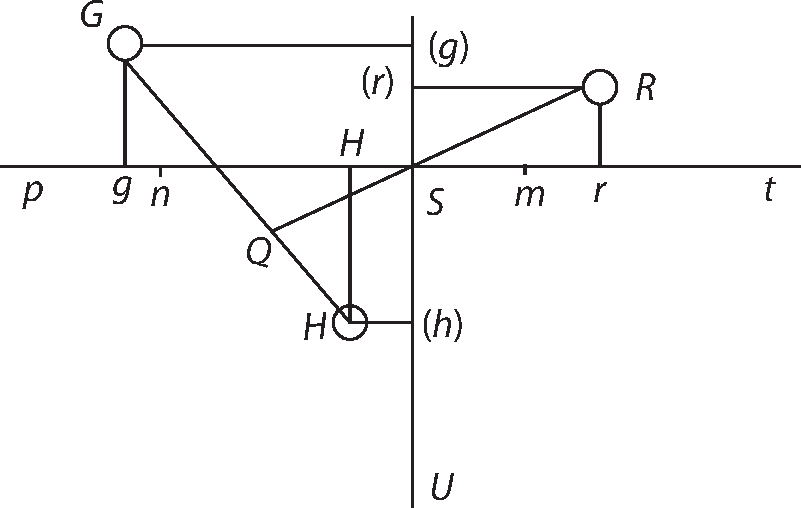
\includegraphics[width=0.57\textwidth]{gesamttex/edit_VIII,3/images/LH_38_212-215_d7_214r.pdf}}
\vspace{0.5em}
\centerline{\lbrack\textit{Fig.~7}\rbrack}
\vspace{1.5em}
%
\pstart
\noindent \textit{des} \edtext{C.~9.}{%
\lemma{\hspace{1.6mm}%
\lbrack\textit{Fig.~7}\rbrack%
}\killnumber%
\Cfootnote{%
tlw.\ Übernahme der Vorlage: a.a.O., Pl.~3, Fig.~41.%
}}
%
\edtext{\textit{corps \textit{G}, \textit{H}, \textit{R}}}{\lemma{\textit{corps}}\Bfootnote{\textit{(1)} \textit{G}, \textit{R} \textit{(2)} \textit{\textit{G}, \textit{H}, \textit{R}} \textit{L}}} 
%
\textit{determinées à agir toutes en même sens, selon les perpendiculaires} 
%
\textit{Gg}, \textit{Hh}, \textit{Rr}; et \textit{menant} \textit{encor}
%
\edtext{\textit{par \textit{S} la parallele}}{\lemma{par \textit{S}}\Bfootnote{\textit{(1)} la paralle \textit{(2)} la \textit{(a)} droi \textit{(b)} parallele \textit{L}}} 
%
à ces \textit{directions} \textit{SU} \textit{et abaissant sur} elle les \textit{perpendiculaires} \textit{G}(\textit{g}), \textit{H}(\textit{h}), \textit{R}(\textit{r}) 
%
(\protect\vphantom)+ je me sers des
%
\edtext{notes \textit{H}, \textit{h}, (\textit{h})}{\lemma{notes}\Bfootnote{\textit{(1)} \textit{R}, \textit{r}, (\textit{r}), car l'auteur prend \textit{(2)} \textit{H}, \textit{h}, (\textit{h}) \textit{L}}} 
%
car l'auteur prend \textit{H}, \textit{q}, \textit{n} +\protect\vphantom() 
%
\textit{on verra par ce qu'on a dit du centre\protect\index{Sachverzeichnis}{centre de masse} de masse} 
%
(+ gravité\protect\index{Sachverzeichnis}{centre de gravité} +) 
%
\textit{que la somme des momens de} \textit{Sg} \textit{par la force de \textit{G}}, et \textit{Hh} \textit{par la force de} \textit{H}, \textit{sera}
%
\edtext{\textit{egale} au moment}{\lemma{\textit{egale}}\Bfootnote{\textit{(1)} \textit{à} la force \textit{(2)} au moment \textit{L}}} 
%
de \textit{Sr par la force} de \textit{R}. \textit{En sorte que si \textit{H}} estoit \textit{de l'autre costé de}
%
\edtext{\textit{pt} \textit{à}}{\lemma{\textit{pt}}\Bfootnote{\textit{(1)}~que \textit{(2)} \textit{à} \textit{L}}} 
%
\textit{l'egard de \textit{G} et} \textit{R} \textit{on suppose \textit{G}, \textit{R}, 
%
pousser les points} \textit{g}, \textit{r}, et \textit{H} \textit{tirer} le point \textit{h}, \textit{il y aura}
%
\edtext{\textit{equilibre} \textit{S}.\edlabel{38_212-215_3b} (\protect\vphantom)+ Il faut}{\lemma{\textit{equilibre} \textit{S}.}\Bfootnote{\textit{(1)} (\protect\vphantom)+ Cela me paroist obscur \textit{(2)} (\protect\vphantom)+ Il faut \textit{L}}}
%
que \textit{H} tire, à fin que
%
\edtext{tous trois}{\lemma{tous}\Bfootnote{\textit{(1)}~tendent \textit{(2)} trois \textit{L}}} 
%
points tendent du même costé. Et il faut s'imaginer que la ligne \textit{pt}
%
\edtext{soit rigide}{\lemma{soit}\Bfootnote{\textit{(1)} mobile \textit{(2)} rigide \textit{L}}} 
%
mobile à l'entour du point \textit{S}. 
%
\edtext{L'auteur dit que ce centre de force\protect\index{Sachverzeichnis}{centre de force} est ce qu'on appelloit autres fois centre de percussion\protect\index{Sachverzeichnis}{centre de percussion};}{%
\lemma{L'auteur \lbrack...\rbrack\ percussion}%
\Cfootnote{%
a.a.O., S.~110;\cite{01500}
siehe auch
\protect\index{Namensregister}{\textso{Wallis} (Wallisius), John 1616\textendash1703}\textsc{J.~Wallis}, \cite{00301}\textit{Mechanica}, London 1670\textendash1671, Pars~III, Cap.~XI, Prop.~XV S.~677\textendash682 (\cite{01008}\textit{WO} I, S.~1012\textendash1015)
und
\protect\index{Namensregister}{\textso{Mariotte}, Edme, Seigneur de Chazeuil ca. 1620\textendash1684}
\textsc{E.~Mariotte}, \cite{00311}\textit{Traité de la percussion}, Paris 1673, 
Seconde partie, Prop.~XIV,
S.~267\textendash271.}}
%
et que si on applique une force contraire
%
\edtext{egale}{\lemma{}\Bfootnote{egale \textit{erg. L}}} 
%
en \textit{S}, supposant la connexion des corps en \textit{S}, on les y arreste. Aussi est ce là, où ils agissent
%
\edtext{avec tout}{\lemma{avec}\Bfootnote{\textit{(1)}~toute leur force \textit{(2)} tout \textit{L}}}
%
leur effort.
\pend
\newpage
\pstart
Ch.\
%
\edtext{\lbrack 11.\rbrack}{\lemma{}\Bfootnote{9. \textit{L ändert Hrsg.}}} 
%
\edlabel{38_212-215_11a}%
\edtext{}{% C-Footnote
{\xxref%
{38_212-215_11a}{38_212-215_11b}}%
\lemma{Si \lbrack...\rbrack\ force}%
\Cfootnote{%
\textsc{Parent}, \textit{Élémens}, S.~114\textendash117.\cite{01500}%
}}%
Si les
%
\edtext{corps \textit{G}, \textit{R},}{\lemma{corps}\Bfootnote{\textit{(1)} \textit{G}, \textit{H} \textit{(2)} \textit{G}, \textit{R}, \textit{L}}} 
%
(omettant \textit{H}, comme s'il n'y estoit point) 
%
choquoient la verge \textit{pt}, en \textit{g}, et \textit{r}, et que le point \textit{S}, estoit le centre de
%
\edtext{percussion, et qu'il}{\lemma{percussion,}\Bfootnote{\textit{(1)} il est clair que tout leur \textit{(2)} et \textit{(a)} qu'il \textit{(b)} qu'il \textit{L}}} 
%
y eût là un appuy, tout de même seroit en
%
\edtext{equilibre\protect\index{Sachverzeichnis}{equilibre}. S'il y avoit deux appuis, 
\textit{S}}{\lemma{equilibre.}\Bfootnote{\textit{(1)} Mais si l'app \textit{(2)} S'il y avoit deux appuis, \textit{(a)} \textit{m}, \textit{n}, hors de \textit{S} \textit{(b)} \textit{S} \textit{L}}} 
%
et \textit{m}, l'appuy \textit{m} seroit inutile, tout estant soutenu en \textit{s}.
%
Mais si les deux appuys estoient \textit{m}
%
\edtext{et \textit{n} pour}{\lemma{et \textit{n}}\Bfootnote{\textit{(1)} on peut s'imaginer \textit{(2)} pour \textit{L}}} 
%
sçavoir combien un des appuys, par exemple \textit{n}, est chargé, on le peut considerer comme une puissance 
%
qui doit soutenir le choc des corps \textit{G}, \textit{R}, en \textit{g} et \textit{r}, lors qu'ils font effort 
%
de mouvoir centralement la verge \textit{pt}, à l'entour de \textit{m} 
%
(\protect\vphantom)+ quoyque icy le corps \textit{R} le charge negativement, c'est à dire il l'aide +\protect\vphantom(), 
%
l'auteur conclut que les efforts que portent les appuys \textit{m} et \textit{n}, sont entre eux comme \textit{Sn} à \textit{Sm}, c'est à dire
%
%
\edlabel{38_212-215_4a}%
\edtext{}{%
{\xxref%
{38_212-215_4a}{38_212-215_4b}}%
\lemma{reciproquement.}\Bfootnote{%
\textit{(1)} (\protect\vphantom)+ Il ne dit p 
\textit{(2)} L'effort même \textit{(a)} est \textit{(b)} sur \textit{n} est 
\textit{(3)} L'effort sur l'appuy \textit{n} est 
\textit{(a)} \textit{G}.
\textit{(b)} \textit{Gg} 
\textit{(c)} \textit{G}.\ en vistesse de \textit{G}.\ en $gm-R$, en vistesse de \textit{R}.\ en \textit{rm}  ce qui seroit egal à \textit{n}.\ en vistesse de \textit{N}.\ en \textit{nm} supposant que \textit{n} au lieu d'appuy soit un un corps agissant d'un effort contraire pour soutenir ce que l'appuy 
\textit{(4)} Si \textit{L}}}%
reciproquement. %
\pend
%
\vspace{1.5em}
\centerline{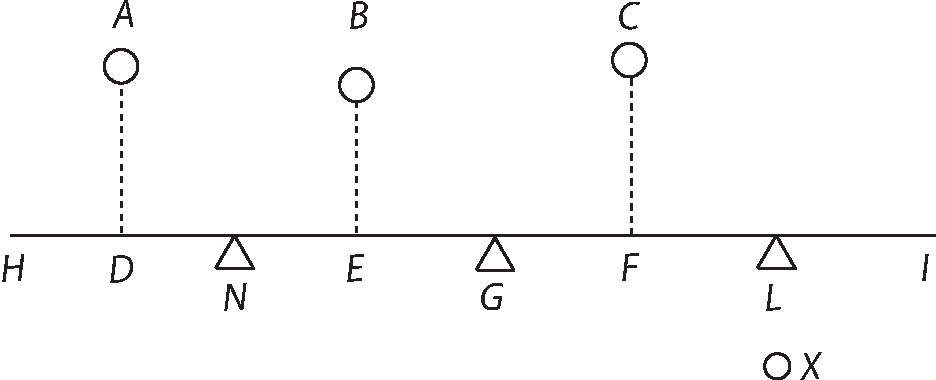
\includegraphics[width=0.67\textwidth]{gesamttex/edit_VIII,3/images/LH_38_212-215_d8_214r.pdf}}
\vspace{0.5em}
\centerline{\lbrack\textit{Fig.~8}\rbrack}
\vspace{1.0em}
%
\pstart
\edtext{Si\edlabel{38_212-215_4b}}{%
\lemma{\hspace{1,6mm}%
\lbrack\textit{Fig.~8}\rbrack%
}\killnumber%
\Cfootnote{%
tlw.\ Übernahme der Vorlage: a.a.O., Pl.~3, Fig.~43.\cite{01500}%
}}
%
$A\cdot AD \cdot DG+B\cdot BE \cdot EG = C\cdot CF \cdot FG$ supposé que les distances des corps 
%
de la verge \textit{HI} representent les vistesses du choc, alors \textit{G} est le point 
%
d'equilibre\protect\index{Sachverzeichnis}{point d'equilibre} d'effort, ou le centre de 
%
percussion\protect\index{Sachverzeichnis}{centre de percussion}. Que si au lieu de cela il y avoit deux 
%
appuys \textit{L} et \textit{N} et qu'on voulut sçavoir combien l'appuy est chargé il faut considerer la verge
%
\textit{HI} mobile sur \textit{N}, et poussée par \textit{A}, \textit{B}, \textit{C}, selon
%
\edtext{leur\lbrack s\rbrack}{\lemma{}\Bfootnote{leur \textit{L ändert Hrsg.}}} 
%
directions et combien il faudroit qu'un corps en \textit{Q} eut d'effort pour y resister. 
%
Cet effort doit estre $-A\cdot AD\cdot DN+B\cdot BE\cdot EN+C\cdot CF\cdot FN$. 
%
Si le corps resistant estoit \textit{X} il y auroit $X\cdot XL\cdot LN$. 
%
Et $X\cdot XL$ effort du corps en luy même, est 
%
$-A\cdot AD\cdot DN+B\cdot BE\cdot EN+C\cdot CF\cdot FN,:LN$. 
%
Mais $-A\cdot AD\cdot DN+B\cdot BE\cdot EN +C\cdot CF\cdot FN$ 
%
est $=A\cdot AD+B\cdot BE+C\cdot CF, GN$, par la nature du centre de force\protect\index{Sachverzeichnis}{centre de force} ou de
%
percussion.\protect\index{Sachverzeichnis}{centre de percussion} Donc nous aurons
%
$A\cdot AD+B\cdot BE+C\cdot CF,$
%
\edtext{$GN:LN$. C'est}{\lemma{$GN:LN$.}\Bfootnote{\textit{(1)} et à l'egard de l'appuy \textit{L} ce qui souffre \textit{(2)} C'est \textit{L}}} 
%
ce que souffre l'appuy \textit{L}; c'est pourquoy pour sçavoir ce qui souffre l'appuy \textit{N}, 
%
on n'a qu'à mettre \textit{GL} au lieu de \textit{GN}. La somme des deux efforts que souffrent \textit{L} et 
%
\textit{N}, est la même que celle que souffre l'appuy \textit{G}, c'est à dire le centre de force.%
\edlabel{38_212-215_11b}
%
(\protect\vphantom)+ Que dirons nous s'il y avoit trois appuys? En \textit{N}, \textit{L},
%
\edtext{\textit{I}. Je diray}{\lemma{\textit{I}.}\Bfootnote{\textit{(1)} Il semble \textit{(2)} Je diray~\textit{L}}} 
%
que l'appuy \textit{N} sera chargé, comme si l'appuy \textit{I} n'y estoit
%
\edtext{pas; et de}{\lemma{pas;}\Bfootnote{\textit{(1)} à l'egard des chocs qui tombent entre \textit{N} et \textit{L}, mais \textit{(2)} et de \textit{L}}} 
%
même l'appuy \textit{I} comme si l'appuy \textit{N} n'y estoit pas. 
%
Mais comment sera chargé l'appuy \textit{L}? Qui est au milieu. On dira que non. Mais c'est une
%
\edtext{erreur puisqu'il}{\lemma{erreur}\Bfootnote{\textit{(1)} puisque \textit{(2)} puisqu'il \textit{L}}} 
%
faut bien qu'il souffre, \textit{N}, ne souffrant qu'autant que \textit{L} soutient. Ainsi tous ces raisonnemens ne sont point
%
\edtext{solides. Ce}{\lemma{solides.}\Bfootnote{\textit{(1)} le veritables \textit{\lbrack\!!\rbrack} \textit{(2)} Ce \textit{L}}} 
%
que souffrent les appuys est toute autre chose. Car c'est une force vive\protect\index{Sachverzeichnis}{force vive}, 
%
sçavoir toute la compression faite par le choc 
%
et par consequent elle a de tout autres loix. Mais autre chose est, quand au lieu des appuys 
%
on prend des corps choquans contraires. Mais il en faudroit considerer aussi la compression. +\protect\vphantom() 
\lbrack214~v\textsuperscript{o}\rbrack\ 
\pend
%214v
%
\vspace{1.5em}
\centerline{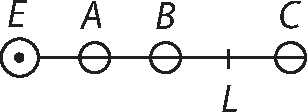
\includegraphics[width=0.23\textwidth]{gesamttex/edit_VIII,3/images/LH_38_212-215_d9_214v.pdf}}
\vspace{0.5em}
\centerline{\lbrack\textit{Fig.~9}\rbrack}
\vspace{1.0em}
%
%
\pstart 
\edtext{Ch.~12.}{%
\lemma{\hspace{1,6mm}%
\lbrack\textit{Fig.~9}\rbrack%
}\killnumber%
\Cfootnote{%
tlw.\ Übernahme der Vorlage: a.a.O., Pl.~3, Fig.~44.%
}}
%
%
%
\edlabel{38_212-215_5a}%
\edtext{}{%
{\xxref%
{38_212-215_5a}{38_212-215_5b}}%
\lemma{\textit{Centre virtuel de force}}\Cfootnote{a.a.O., S.~117.\cite{01500}}}%
\textit{Centre virtuel de}
%
\edtext{\textit{force}.%
\edlabel{38_212-215_5b}
Supposons}{\lemma{\textit{force}.}\Bfootnote{\textit{(1)} Le point \textit{C} \textit{(2)} Supposons \textit{L}}} 
%
que les corps \textit{A}, \textit{B}, \textit{C}, choquent le rayon \textit{EL} mobile à l'entour du centre fixe
%
\edtext{\textit{E}, et le}{\lemma{\textit{E}, et}\Bfootnote{\textit{(1)} que \textit{(2)} le \textit{L}}} 
%
point \textit{L} soit tel, que sa vitesse
%
\edtext{circulaire}{\lemma{}\Bfootnote{circulaire \textit{erg. L}}} 
%
qu'il aura après le
%
choc
%
\edtext{à l'entour}{%
\lemma{}%
\Bfootnote{%
à l'entour %
\textit{erg.~ L}%
}}
%
estant donnée à toute la masse des corps ce 
%
\edtext{\textit{moment total sera egal à la somme des} \edtext{\textit{momens} de}{\lemma{\textit{momens}}\Bfootnote{\textit{(1)} après le choc \textit{(2)} de \textit{L}}} tous les \textit{corps après le choc}.}{%
\lemma{\textit{moment} \lbrack...\rbrack\ \textit{choc}}%
\Cfootnote{%
a.a.O., S.~118.\cite{01500}
%
}}
%
(+ Est ce le centre de force futur? +) 
%
\edtext{Il donne la regle pour le trouver,}{%
\lemma{Il donne \lbrack...\rbrack\ trouver}%
\Cfootnote{%
a.a.O., S.~118.\cite{01500}
%
}}
%
mais il y a fautes d'impression non corrigées qui rendent le tout obscur. 
%
\pend 
\newpage
%
%
\pstart
%
Ch.
%
\edtext{%
\edtext{13.\ \textit{Des chocs}}{\lemma{13.}\Bfootnote{\textit{(1)} Tout corp \textit{(2)} \textit{Des chocs} \textit{L}}}
%
\textit{dans tous les points d'un corps.}%
}{%
\lemma{\textit{Des chocs} \lbrack...\rbrack\ \textit{corps}}%
\Cfootnote{%
a.a.O., S.~119.\cite{01500}\hspace{10mm}%
}} 
%
Un corps se mouvant
%
\edtext{parallel\lbrack eme\rbrack nt}{\lemma{}\Bfootnote{parallelant \textit{L ändert Hrsg.}}}, c'est à dire en sorte que \textit{toutes}\edlabel{38_212-215_214v1}
%
\edtext{\textit{les parti}\lbrack\textit{e}\rbrack\textit{s} \textit{se}}{\lemma{}\Bfootnote{%
\textit{les} \textbar\ partis \textit{ändert Hrsg. nach Vorlage} \textbar\ \textit{se} \textit{L}}}
\textit{meuvent avec}
%
\edtext{\textit{des} \lbrack\textit{vitesses}\rbrack\ \textit{directes}}{\lemma{}\Bfootnote{%
\textit{des} \textbar\ parties \textit{ändert Hrsg. nach Vorlage} \textbar\ \textit{directes} \textit{L}}}
\textit{et egales}, alors le centre de Masse et le centre de force sont les mêmes.
%
\edtext{Si un plan}{\lemma{Si}\Bfootnote{\textit{(1)} le corps \textit{(2)} un plan \textit{L}}}
se meut en sorte qu'un point fixe
%
\edtext{dans ce plan\lbrack,\rbrack}{\lemma{dans ce}\Bfootnote{\textit{(1)} corps \textit{(2)} plan \textit{L}}}
procede par une ligne courbe
%
\edtext{tousjours \textit{perpendiculaire}}{\lemma{tousjours}\Bfootnote{\textit{(1)} parallele \textit{(2)}~\textit{perpendiculaire} \textit{L}}}
\textit{à} ce \textit{plan les autres points allant inegalement viste, mais tous}jours \textit{parallelement entre eux; elle a un centre\protect\index{Sachverzeichnis}{centre de force} de force} 
%
(\protect\vphantom)+ les lignes descrites ne sont point paralleles entre elles, mais les directions des points 
%
sont tousjours paralleles +\protect\vphantom() 
%
qui sera alors different du centre de masse\protect\index{Sachverzeichnis}{centre de masse}, si le corps ne
%
\edtext{rencontre un obstacle}{\lemma{rencontre}\Bfootnote{\textit{(1)} point \textit{(2)} un obstacle \textit{L}}}
hors \textit{du chemin de son centre de \edlabel{38_212-215_214v2}masse}\edtext{}{{\xxref{38_212-215_214v1}{38_212-215_214v2}}\lemma{\textit{toutes les}  \lbrack...\rbrack\ \textit{centre de masse}}\Cfootnote{a.a.O., S. 119.\cite{01500}}}, il fait effort de tourner à l'entour du point qu'il rencontre. 
\pend 
\pstart 
Ch.~14. 
\edtext{Du centre\protect\index{Sachverzeichnis}{centre de temps} \textit{de temps}.
%
Les corps \textit{L}, \textit{M}, \textit{N},
%
\edtext{\textit{Q} vont}{\lemma{}\Bfootnote{\textit{Q}  \textbar\ attachés à \textit{(1)} 7\textit{A}234 \textit{(2)} la verge 7\textit{A}234 \textit{erg. u. gestr.} \textbar\ vont \textit{L}}}
de 2, 3, 4, 7 en \textit{Y}, \textit{Z}, \textit{K}, \textit{R}
%
\edtext{par des arcs decrits à l'entour du centre \textit{A}, sçavoir 2\textit{Y}, 3\textit{Z}, 4\textit{K}, 7\textit{R}}{\lemma{}\Bfootnote{par des  \lbrack...\rbrack\ 4\textit{K}, 7\textit{R} \textit{erg. L}}}
dans les temps representés \textit{par les ordonnées}
%
2\textit{E}, 3\textit{F}, 4\textit{G}, ainsi ces temps estant inegaux, les corps sont libres dans ce}{%
\lemma{Du centre \lbrack...\rbrack\ mouvement}%
\Cfootnote{%
a.a.O., S. 122.\cite{01500}%
}}%
\edlabel{KZeitz107}\edtext{}{{\xxref{KZeitz107}{KZeitz108}}%
{%
\lemma{Concevons \lbrack...\rbrack\ temps}%
\Cfootnote{%
a.a.O., S. 123.\cite{01500}%
}}}
\edtext{mouvement. Concevons}{\lemma{mouvement.}\Bfootnote{\textit{(1)} Soit 3\textit{F} le temps, \textit{(2)} Concevons \textit{L}}} 
maintenant que les corps \textit{L}, \textit{M}, \textit{N}, \textit{Q}, choquent les\edtext{}{%
\lemma{\hspace{1,6mm}%
\lbrack\textit{Fig.~10}\rbrack%
}\killnumber%
\Cfootnote{%
tlw.\ Übernahme der Vorlage: a.a.O., Pl.~3, Fig.~46.\cite{01500}%
}}%
\pend
%
\vspace{1.2em}
\centerline{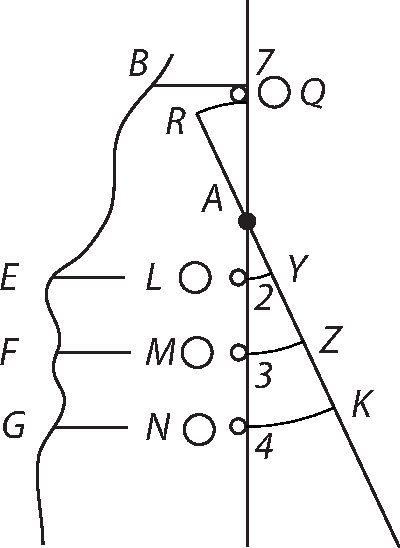
\includegraphics[width=0.28\textwidth]{gesamttex/edit_VIII,3/images/LH_38_212-215_d10_214v.pdf}}
\vspace{0.5em}
\centerline{\lbrack\textit{Fig.~10}\rbrack}
%\vspace{1.0em}
%
\newpage
\pstart
\noindent les corps 2, 3, 4, 7 
(egaux à \textit{L}, \textit{M}, \textit{N}, \textit{Q}) que le rayon solide 74 \textit{porte, pour les faire} 
%
\edtext{\textit{arriver} avec}{%
\lemma{\textit{arriver}}%
\Bfootnote{%
\textit{(1)} à la situa %
\textit{(2)} avec %
\textit{L}%
}}
%
leur rayon \textit{à la situation RAK, dans un certain temps} qui soit par exemple 3\textit{F}. Alors on appellera 3 
%
\textso{\textit{le centre de} }\edtext{\textso{\textit{temps}}.
%
Si}{\lemma{\textso{\textit{temps}}.}\Bfootnote{\textit{(1)} Si pas un des co \textit{(2)} Si \textit{L}}} 
%
le temps de pas un des corps y repondoit, il n'y auroit point de centre de temps.\edlabel{KZeitz108}
%
(\protect\vphantom)+ Mais lors qu'il y a une infinite de mobiles comme si le rayon même estoit le corps d'inegale grosseur,
%
il y auroit tousjours le Centre de temps. +\protect\vphantom() 
%
Il peut y avoir plusieurs centres de temps à la fois, lors que plusieurs corps arrivent en même temps. 
%
\edtext{Si \textit{les corps}	%
%
\edtext{\textit{choquans ont}}{%
\lemma{\textit{choquans}}%
\Bfootnote{%
\textit{(1)}~\textbar\ sont proportionnels \textit{streicht Hrsg.}\ \textbar\ %
\textit{(2)} \textit{ont} \textit{L}}}%
\textit{des vistesses egales et sont}
%
\edtext{\textit{proportion}\lbrack\textit{n}\rbrack\textit{els}}{\lemma{}\Bfootnote{proportionels \textit{ L ändert Hrsg.}}} 
%
\textit{aux corps choqués}\lbrack,\rbrack\ item si 
%
\textit{les corps choquans n'ont ny l'un ny l'autre et}
%
\edtext{\textit{doivent cependant}}{\lemma{\textit{doivent}}\Bfootnote{\textit{(1)}~neantmoins \textit{(2)} \textit{cependant} \textit{L}}} 
%
\textit{donner des vistesses egales aux corps choqués};%
}{%	
\lemma{Si \lbrack...\rbrack\ \textit{choqués}}%
\Cfootnote{%
a.a.O., S.~124.\cite{01500}\hspace{20mm}%
}}
%
\edtext{\textit{le centre des temps est} aussi \textit{le centre de force} du tout \textit{après le choc}.}{%
\lemma{\textit{le centre des temps} \lbrack...\rbrack\ \textit{choc}}%
\Cfootnote{%
a.a.O., S.~127.\cite{01500}%
}}
%
Generalement le
%
\edtext{\textit{centre de temps est le même que ce qu'on a} appellé \textit{dans la pesanteur le centre d'oscillation}}{\lemma{\textit{centre}  \lbrack...\rbrack\ \textit{d'oscillation}}\Cfootnote{a.a.O., S.~127.\cite{01500}}}.
\pend
%
\pstart Ch.~15
%
\edtext{\textit{Une des experiences qui me semble faire connoistre plus à fonds la nature de la pesanteur, 
%
est celle qui fait voir que le centre\protect\index{Sachverzeichnis}{centre de temps} de temps}}{\lemma{\textit{Une des}  \lbrack...\rbrack\ \textit{centre de temps}}\Cfootnote{a.a.O., S.~127.\cite{01500}}} 
%
(+ centre d'oscillation\protect\index{Sachverzeichnis}{centre d'oscillation} \lbrack+\rbrack) est le 
%
\edtext{même que le centre}{\lemma{même}\Bfootnote{que \textit{(1)} celuy \textit{(2)} le centre \textit{L}}} 
%
de Force (+ centre de percussion\protect\index{Sachverzeichnis}{centre de percussion} +).
%
(\protect\vphantom)+ 
%
\edtext{C'est Monsieur Mariotte\protect\index{Namensregister}{\textso{Mariotte}, Edme, Seigneur de Chazeuil ca. 1620\textendash1684}
%
qui a deja monstré que le centre de percussion est le même avec le centre d'oscillation que 
%
\protect\index{Namensregister}{\textso{Huygens} (Hugenius, Ugenius, Hugens, Huguens), Christiaan 1629\textendash1695}M.~Hugens avoit expliqué.}{%
\lemma{C'est \lbrack...\rbrack\ expliqué}%
\Cfootnote{%
\textsc{Mariotte},
\cite{00311}\title{Traité de la percussion}, %
Seconde partie, Prop.~XIX,
S.~288\textendash\lbrack291\rbrack;
\protect\index{Namensregister}{\textso{Huygens} (Hugenius, Ugenius, Hugens, Huguens), Christiaan 1629\textendash1695}%
\textsc{C.~Huygens}, %
\cite{00123}\title{Horologium Oscillatorium}, 	
 Paris 1673, Pars IV, S.~91\textendash156 %
(\cite{00113}\textit{HO} %
XVIII, S.~242\textendash359).}}
%
Je ne voy pas que cela serve beaucoup à faire connoistre la nature de la pesanteur. 
%
On peut connoistre ces choses par demonstration independemment de l'experience 
%
supposant seulement l'acceleration\protect\index{Sachverzeichnis}{acceleration uniforme} uniforme. +\protect\vphantom() \textit{On}\edlabel{38_212-215_214v5}
%
\edtext{\textit{explique} les \textit{vistesses}}{\lemma{\textit{explique}}\Bfootnote{\textit{(1)} toute \textit{(2)} les \textit{vistesses} \textit{L}}} 
%
\textit{egales des corps} pesans \textit{au commencement de leur} descente, 
%
\textit{en supposant que les corps qui les choquent leur sont proportionnels et ont chacun 
%
une même vistesse} (par le chap.\ precedent) et c'est ce qu'on comprend de la \textit{matiere fluide}, 
%
\edtext{dont tousjours}{%
\lemma{dont}%
\Bfootnote{%
\textit{(1)} la viste %
\textit{(2)} tousjours %
\textit{L}%
}}
%
\textit{un volume proportionnel} est \textit{appliqué} au corps 
%
(+ on peut supposer que ceux qui sont plus rares sont plus percés à jour \lbrack+\rbrack) 
%
\textit{et dont la vitesse est tousjours la même}. L'auteur conclut que les
%
\edtext{proprietes de}{\lemma{proprietes}\Bfootnote{\textit{(1)} des corps ont \textit{(2)}~de \textit{L}}} 
%
la pesanteur ont este connues \textit{par l'experience mais doute qu'on peut dire que la cause} en \textit{a esté ignorée \edlabel{38_212-215_214v6}jusqu'icy}\edtext{}{{\xxref{38_212-215_214v5}{38_212-215_214v6}}\lemma{\textit{On explique}  \lbrack...\rbrack\ \textit{jusqu'icy}}\Cfootnote{\textsc{Parent}, \textit{Élémens}, S. 130f. mit Auslassung.\cite{01500}}}.
\pend
\newpage
%
\pstart 
%
Ch.~17. Il est dit à la fin de ce chapitre: qu'on peut demander 
%
\edlabel{38_212-215_214v7}%
\edtext{}{{\xxref{38_212-215_214v7}{38_212-215_214v8}}\lemma{\textit{plusieurs}  \lbrack...\rbrack\ \textit{Cycloide}}\Cfootnote{a.a.O., S.~140.\cite{01500}}}%
%
\textit{plusieurs questions curieuses, comme} par exemple \textit{le}
%
\edtext{\textit{rayon de la}}{\lemma{\textit{rayon de}}\Bfootnote{\textit{(1)} l'isochrone \textit{(2)} \textit{la} \textit{L}}} 
%
\textit{developpée qui est isochrone à toute la ligne parcourue, en sorte}
%
\edtext{\textit{que} le}{\lemma{\textit{que}}\Bfootnote{\textit{(1)} \textit{O} seroit \textit{(2)} le \textit{L}}} 
%
point \textit{O} de la developpee \textit{seroit un centre et \textit{OG}} (le fil produit jusqu'à la ligne decrite par le developpement) 
%
\textit{un rayon d'une nouvelle espece}. (+ Je crois qu'il veut dire dont le centre change. +) 
%
\textit{De plus quelle est la ligne entre deux points donnés dont le rayon d'oscillation\protect\index{Sachverzeichnis}{rayon d'oscillation} est le plus court. 
%
On a deja determiné que c'est la \edlabel{38_212-215_214v8}Cycloide}\lbrack,\rbrack\
%
pag.~140. (+ où? +) \pend
%
\pstart Troisieme partie chap.~1.
%
\edtext{\textit{Des mouvemens et des forces\protect\index{Sachverzeichnis}{force relative} relatives} 
%
et \textit{derivées}.}{\lemma{\textit{Des}  \lbrack...\rbrack\ \textit{derivées}}\Cfootnote{a.a.O., S.~148.\cite{01500}}}
%
\edlabel{38_212-215_12a}%
\edtext{}{% C-Footnote 
{\xxref%
{38_212-215_12a}{38_212-215_12b}}%
\lemma{}%
\Cfootnote{%
\hspace{-2.4mm}L'auteur \lbrack...\rbrack\ droite: \hspace{0.1mm}a.a.O., S.~149\textendash151.\cite{01500}%
}}%
L'auteur prend pour accordé que les courbes ne sont que des lignes droites infiniment petites, 
%
et que le corps tend tousjours en ligne droite, à moins qu'il  en soit detourné continuellement. 
%
\pend
%
%
\vspace{1.5em} %%%%%%%%% Diagramm 11
\centerline{%
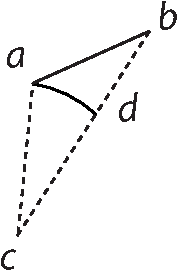
\includegraphics[width=0.14\textwidth]{%
gesamttex/edit_VIII,3/images/LH_38_212-215_d11_214v.pdf%
}} 
\vspace{0.5em}
\centerline{%
\lbrack\textit{Fig.~11}\rbrack%
}
% \newpage%
\vspace{1.0em}
%
%
\pstart 
Un point allant d'\textit{a} en \textit{b}, s'eloigne d'\textit{a} de la quantite
%
\edtext{\textit{ab}, qu'on peut}{\lemma{\textit{ab}}\Bfootnote{\textit{(1)} mais on pe \textit{(2)}~qu'on peut \textit{L}}} 
%
appeller son mouvement positif, mais si on tire du point \textit{c} les droites \textit{ca}, \textit{cb}, 
%
et que du centre \textit{c} on decrit l'arc \textit{ad}, coupant \textit{cb} en \textit{d}, on voit que le mobile 
%
s'est eloigné de \textit{c}, de la quantite \textit{db}, et qu'il a aussi decrit l'arc \textit{ad}, à l'entour de \textit{c}.
%
Et \textit{ab} estant infiniment petite, ou élement d'une courbe, l'arc \textit{ad} ne differera point 
%
de la droite.\edlabel{38_212-215_12b} 
\pend
%
%
\pstart
Ch.~3. 
%
Il n'y a que \textit{deux\edlabel{38_212-215_214v9} cas}\edtext{}{{\xxref{38_212-215_214v9}{38_212-215_214v10}}\lemma{\textit{deux}  \lbrack...\rbrack\ \textit{choc}}\Cfootnote{a.a.O., S.~158 mit Auslassungen.\cite{01500}}} 
%
\textit{où les forces derivées\protect\index{Sachverzeichnis}{force derivée} sont les mêmes que les 
%
composantes\protect\index{Sachverzeichnis}{force composante}}. C'est lors que le parallelogramme des 
%
forces composées devient un rectangle, ou les trois directions font 
%
un parallelepipede rectangle. Car
%
\edtext{quoyque deux}{\lemma{quoyque}\Bfootnote{\textit{(1)} le corps \textit{A} soit \textit{(2)} deux  \textit{L}}} 
%
corps soyent capables de donner à un
%
\edtext{troisieme chacun separement sa vistesse}{\lemma{troisieme}\Bfootnote{\textit{(1)} deux vistesses \textit{(2)}~chacun separement sa vistesse \textit{L}}},
%
 il ne faut point imaginer qu'ils les luy donnent aussi conjointement. 
%
\textit{Car si on me dit qu'il satisfait par là, à ce que luy de-}
\pend
\newpage
\pstart
\noindent \textit{mandent tous ces corps} joint 
%
ensemble, je dis que les corps ne demandent que ce qu'ordonnent 
%
les loix du choc\edlabel{38_212-215_214v10}, les 
%
\edtext{quelles ordonnent autre chose. Ces}{\lemma{quelles}\Bfootnote{ordonnent \textit{(1)} autres \textit{(2)} autre chose. \textit{(a)} Deux \textit{(b)} Ces \textit{L}}} 
%
directions perpendiculaires entre elles ne s'aident ou ne se diminuent point comme font les l'obliques, 
%
l'obliquite aigue aide, l'obtuse diminue. (\protect\vphantom)+ Verum, car l'aigue aide
%
à éloigner du sens opposé; et l'obtuse porte à l'opposé. \lbrack+\protect\vphantom()\rbrack\ 
%
(\protect\vphantom)+ Et cette oblique 
%
\edtext{\textit{AC}}{%
\lemma{}%
\Bfootnote{%
\textit{AC} %
\textit{erg.\ L}%
}}
%
peut estre resolue de 
%
\edtext{nouveau en celle qui aide purement}{\lemma{nouveau}\Bfootnote{en \textit{(1)} celle \textit{(a)} qui \textit{(b)} qui est la même \textit{(2)} celle qui aide \textit{(a)} entierement \textit{(b)} purement \textit{L}}},
%
 c'est à dire qui est parallele, et en celle qui n'aide point du
%
\edtext{tout, ou}{\lemma{tout,}\Bfootnote{\textit{(1)}~et \textit{(2)} ou \textit{L}}} 
%
qui est perpendiculaire. +\protect\vphantom()
\pend
\vspace{1.5em} 
\pstart 
\hspace{18mm}\begin{minipage}[t]{0.5\textwidth}
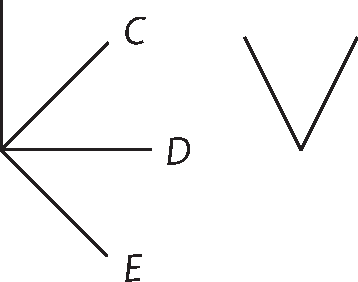
\includegraphics[width=0.4\textwidth]{gesamttex/edit_VIII,3/images/LH_38_212-215_d12_214v.pdf}
\end{minipage}
\hspace{-3mm}
\begin{minipage}[t]{0.5\textwidth}
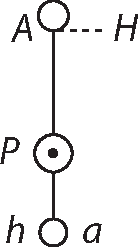
\includegraphics[width=0.2\textwidth]{gesamttex/edit_VIII,3/images/LH_38_212-215_d13_214v.pdf}
\end{minipage}
\\
\\
\hspace*{26mm} [\textit{Fig.~12, gestr.}]\hspace*{40mm} [\textit{Fig.~13}]
\pend
\vspace{1.5em}
%%%
%%%
%%\vspace{1.5em} %%%%%%%%% Diagramm 12, gestr.
%%\centerline{%
%%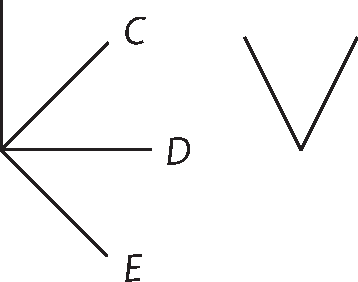
\includegraphics[width=0.21\textwidth]{%
%%gesamttex/edit_VIII,3/images/LH_38_212-215_d12_214v.pdf%	
%%}} 
%%\vspace{0.5em}
%%\centerline{%
%\lbrack\textit{Fig.~12, gestr.}\rbrack%
%}
%% \newpage%
%\vspace{1.0em}
%%
%%
%\vspace{1.5em} %%%%%%%%% Diagramm 13
%\centerline{%
%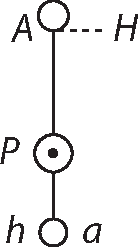
\includegraphics[width=0.1\textwidth]{%
%gesamttex/edit_VIII,3/images/LH_38_212-215_d13_214v.pdf%
%}} 
%\vspace{0.5em}
%\centerline{%
%\lbrack\textit{Fig.~13}\rbrack%
%}
%% \newpage%
%\vspace{1.0em}
%
%
\pstart
Ch.~5. 
%
\setline{8}Du mouvement circulaire. 
%
\edtext{Si une verge \textit{Aa}, tourne à l'entour d'un pivot, comme
%
\edtext{\textit{P}, et porte}{\lemma{\textit{P},}\Bfootnote{\textit{(1)} et \textit{(2)} et que \textit{(3)} et porte \textit{L}}} 
%
les corps \textit{A}, \textit{a} en sorte, que \textit{PA} soit à \textit{Pa} comme \textit{a} à \textit{A}, en sorte que
%
\edtext{les forces}{\lemma{les}\Bfootnote{\textit{(1)} efforts \textit{(2)} forces \textit{L}}} 
%
sont egales (+ efforts egaux +) et qu'on pose que la verge echappe au pivot (\protect\vphantom)en descendant par exemple si ce
%
\edtext{piv\lbrack ot\rbrack}{\lemma{pivoit}\Bfootnote{\textit{L ändert Hrsg.}}} avoit la pointe en
%
\edtext{bas\protect\vphantom() le}{\lemma{bas\protect\vphantom()}\Bfootnote{\textit{(1)} il ne la \textit{(2)} la \textit{(3)} le\textit{L}}} 
%
tour à l'entour du point \textit{P}, dans \textit{Aa}, qui repondoit auparavant au pivot, ne laisseroit pas de 
%
continuer de même. Mais si ces efforts $A\cdot AP$, et $a\cdot ap$ sont inegaux; 
%
et qu'ils tournent à l'entour du pivot \textit{P}, et que la verge avec ces corps echappe par après au pivot, la
%
\edtext{question est à l'entour}{\lemma{question}\Bfootnote{est \textit{(1)} comme \textit{(2)} à l'entour \textit{L}}} 
%
de quel centre ces \edtext{corps}{\lemma{}\Afootnote{\foreignlanguage{ngerman}{\textit{Zwischen \lbrack Fig.~13\rbrack\ und dem Text}:} NB\vspace{-2mm}}} doivent tourner et avec quelle vistesse.}{%
\lemma{Si \lbrack...\rbrack\ vistesse}%
\Cfootnote{%
a.a.O., S.~163\textendash165.\cite{01500}}}
%
 \lbrack(\protect\vphantom)+\rbrack\ L'auteur l'explique d'une maniere qui n'est pas intelligible. 
%
Est ce que leur
%
\edtext{force des}{\lemma{force}\Bfootnote{\textit{(1)} doit employées \textit{(2)} des \textit{L}}} 
%
que la verge est devenue \makebox[1.0\textwidth][s]{libre, doit estre à l'entour de leur centre de 
%
gravite\,\lbrack\!?\rbrack\ 
%
Ita videtur. \textit{A} tachera d'aller le}
\pend
\newpage
\pstart
\noindent plus droit qu'il pourra, aussi tost que \textit{Aa} sera libre, c'est à dire qu'il tachera d'aller vers 
%
\textit{H} avec la vistesse qu'il a et \textit{a} vers \textit{h} aussi avec la sienne, mais l'un empechant l'autre, ils obtiendront le plus 
%
s'ils tournent à l'entour de leur centre de gravité. +\protect\vphantom() 
%
\pend 
%
\vspace{1.5em} %%%%%%%%% Diagramm 14
\centerline{%
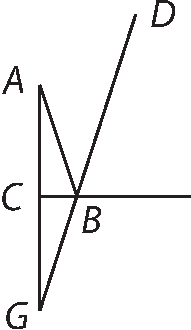
\includegraphics[width=0.14\textwidth]{%
gesamttex/edit_VIII,3/images/LH_38_212-215_d14_214v.pdf%	
}} 
\vspace{0.5em}
\centerline{%
\lbrack\textit{Fig.~14}\rbrack%
}
% \newpage%
\vspace{1.0em}
%
\pstart 
Ch.~6. Pour appliquer la reflexion du plan, à la courbe, il suppose que le plan tangent et la courbe, ont une partie commune. 
%
(\protect\vphantom)+ Mais
%
\edtext{Euclide\protect\index{Namensregister}{\textso{Euklid} (Euclides) von Alexandria 3. Jh. v. Chr.} dit qu'ils n'ont qu'un point commun.}{\lemma{Euclide \lbrack...\rbrack\ commun}%
\Cfootnote{Diese Aussage ist bei \protect\index{Namensregister}{\textso{Euklid} (Euclides) von Alexandria 3. Jh. v. Chr.}Euklid nicht nachweisbar. 
Leibniz meint wohl 
%
\protect\index{Namensregister}{\textso{Archimedes} 287\textendash212 v. Chr.}\textsc{Archimedes}, %
%
\cite{00532}\title{De conoidibus et sphaeroidibus}, Prop.~XVf.}}
%
Ainsi ce raisonnement est susceptible de difficultés, 
%
\edtext{il faut se servir du
\edtext{mien, de la}{\lemma{mien,}\Bfootnote{\textit{(1)} de la \textit{(2)} de ma \textit{(3)} de la \textit{L}}} 
loy de la continuité, où les polygones vont évanouir dans les courbes.%
}{\lemma{il faut \lbrack...\rbrack\ courbes}\Cfootnote{%
Vgl.\ \protect\index{Namensregister}{\textso{Leibniz} (Leibnitius, GGL), Gottfried Wilhelm 1646\textendash1716}\textsc{G.\,W.~Leibniz}, 
\cite{02054}\textit{Extrait d'une lettre de M.~L.\ sur un principe général}, sowie \textsc{Ders.}, \cite{02055}\textit{Principium quoddam generale}.}}
%
+\protect\vphantom()
%
Il est remarquable que toutes les reflechies \textit{BD}, du plan \textit{CB}, quel point que soit \textit{B},
%
concourent toutes au 
%
\edtext{%
point \textit{G}, qu'on peut appeller lieu virtuel de la reflexion.
%
Quant aux courbes il est
%
\edtext{vulgairement}{\lemma{vulgairement}\Bfootnote{\textit{erg. L}}} 
%
connu, qu'il n'y a que le premier hyperboloide ou paraboloide qui donnent un tel lieu virtuel.%
}{%
\lemma{point \textit{G} \lbrack...\rbrack\ virtuel}%
\Cfootnote{%
\cite{01500}\textsc{Parent}, \textit{Élémens}, S.~170.%
}}
\pend
%
\pstart 
%
\hspace{1mm}\hspace{-1mm}% Trick, weil \edlabel nicht zu \par-Beginn sein darf
\edlabel{38_212-215_214v11}%
\edtext{}{{\xxref{38_212-215_214v11}{38_212-215_214v12}}\lemma{\textit{Plusieurs} \lbrack...\rbrack\ \textit{long}}\Cfootnote{a.a.O., S.~170f. mit Auslassung.\cite{01500}}}%
\textit{Plusieurs ont pris pour un principe incontestable de Meta\pgrk{f}ysique qu'un corps qui va} à \textit{un autre par reflexion le doit}
%
\edtext{\textit{faire par le chemin ou}}{\lemma{\textit{faire}}\Bfootnote{\textit{(1)} pour \textit{(2)}~\textit{par le chemin} 
\textit{(a)} le plus court \textit{(b)} \textit{ou} \textit{L}}}
%
\textit{dans le temps le plus court}.
%
 \textit{Mais} dans une \textit{Ellipsoide}, on trouve que 
%
sur la convexe c'est \textit{dans le temps le plus}
%
\edtext{\textit{court}, sur la concave,}{\lemma{\textit{court},}\Bfootnote{sur la \textit{(1)} convexe \textit{(2)} concave, \textit{L}}} 
%
\textit{dans le temps le plus long}.\edlabel{38_212-215_214v12} 
%
Cela peut \edtext{\textit{servir à deprevenir ceux qui pretendent establir les loix de nature}
%
\textit{sur les pures lumieres de leur entendement}.}{%
\lemma{\textit{servir} \lbrack...\rbrack\  \textit{entendement}}%
\Cfootnote{%
a.a.O., S.~170.\cite{01500}%
}}
%
(\protect\vphantom)+ Il est aussi à repondre, 1\textsuperscript{o} qu'on ne l'a pris que comme une hypothese qui a reussi,
%
\edtext{et qu'il}{\lemma{et}\Bfootnote{\textit{(1)}~qu'on \textit{(2)} que \textit{(3)} c'etait necessaire sur les plans \textit{(4)} qu'il \textit{L}}} 
%
falloit l'establir sur les plans, comme c'est en effet une hypothese heureuse, 
%
\edtext{que les mouvemens}{\lemma{que}\Bfootnote{les \textit{(1)} courbes \textit{(2)} mouvemens \textit{L}}} 
%
%215r
\lbrack215~r\textsuperscript{o}\rbrack\ circulaires ont leur direction dans les tangentes\lbrack,\rbrack\ et
%
\edtext{enfin, encor}{\lemma{enfin,}\Bfootnote{\textit{(1)}  qu'il faut \textit{(2)} encor \textit{L}}} 
%
absolument dans les courbes mêmes une maniere de principe a lieu, 
%
c'est que la ligne est la 
%
\edtext{\lbrack plus\rbrack}{%
\lemma{}%
\Bfootnote{%
plus %
\textit{gestr.~L, wieder gültig gemacht Hrsg.}%
}}
%
determinée, ou l'unique. 
%
\lbrack+\protect\vphantom()\rbrack \pend
%
\pstart Ch.~9.
%
\edtext{Si plusieurs corps viennent de tous costés se rendre au point \textit{O},  et que, 
%
\textit{P} soit leur centre de gravite, dont la route soit \textit{PO};}{\lemma{Si  \lbrack...\rbrack\ soit \textit{PO}}\Cfootnote{a.a.O., S.~178.\cite{01500}}} 
%
cette droite \textit{PO} sera tousjours la plus grande. 
%
Et l'effort total des corps estant leur somme par \textit{PO}, il est manifeste, que \textit{PO} est celle 
%
par laquelle cette somme devient la plus grande.
%
\edlabel{38_212-215_6a}Je n'ay pas le loisir d'achever tous ces chapitres comme j'ay commencé.\edlabel{38_212-215_6b}
\pend
%
\pstart 
%
Ch.~13. L'auteur\edlabel{38_212-215_215r1} remarque, que si 
%
\edtext{}{{\xxref{38_212-215_215r1}{38_212-215_215r2}}\lemma{L'auteur \lbrack...\rbrack\ point}\Cfootnote{a.a.O., S.~199f.\cite{01500}}}%
%
la matiere est homogene, 
%
le centre de masse garde tousjours sa route et sa vistesse et si les premiers corps de l'univers sont
%
\edtext{homogenes le centre du monde}{\lemma{homogenes}\Bfootnote{\textit{(1)} leur centre n'aura p \textit{(2)} le centre du monde \textit{L}}} 
%
n'aura point changé son mouvement. Les forces relatives ou derivées se conservent encor. Mais les
%
\edtext{forces positives}{\lemma{forces}\Bfootnote{\textit{(1)} absolues \textit{(2)} positives \textit{L}}}
%
ne se conservent point\edlabel{38_212-215_215r2}. 
%
On\edlabel{38_212-215_215r3} les peut augmenter à l'infini par les chocs
%
\edtext{obliques; mais}{\lemma{obliques;}\Bfootnote{\textit{(1)} mais on les pe \textit{(2)} mais  \textit{L}}} 
%
elle se diminue 
%
\edtext{dans les chocs des}{\lemma{dans}\Bfootnote{les \textit{(1)} corps \textit{(2)} chocs \textit{(a)} à ress \textit{(b)} des \textit{L}}} 
%
corps à ressort imparfait\edlabel{38_212-215_215r4}\edtext{}{{\xxref{38_212-215_215r3}{38_212-215_215r4}}\lemma{O}\Cfootnote{\hspace{-2.4mm}n \lbrack...\rbrack\ imparfait: \hspace{1mm}a.a.O., S.~203.\cite{01500}}}. 
\pend
%
\pstart 
%
\edtext{Part. 4. Ch.~3. Il promet un traité des hydrauliques.}{%
\lemma{Part. 4. Ch.~3. \lbrack...\rbrack\ hydrauliques}%
\Cfootnote{%
Eigentlich \cite{01500}chap.~II, S.~290.}}
\pend
%
\pstart Ch.~4. 
%
\edtext{Il est difficile de \textit{mesurer les forces accidentelles par} les \textit{permanentes comme} 
%
les \textit{poids des animaux}, car \textit{tout corps choquant un poids} de grandeur quelconque, l'eleve tant soit peu. 
%
C'est pour cela, qu'on pourroit \textit{faire choquer} un \textit{corps en mouvement contre un marbre poli} 
%
ou \textit{collé contre un autre marbre, ou faire casser quelque corps inflexible}.}{\lemma{Il \lbrack...\rbrack\ \textit{inflexible}}\Cfootnote{a.a.O., S.~314f. mit Auslassungen.\cite{01500}}} 
%
\pend
%
\pstart Ch.~7. Traitant
%
des corps flexibles non extendibles, et 
%
\edtext{disant que la somme des
%
\edtext{elemens de la courbe}{%
\lemma{elemens}%
\Bfootnote{de %
\textit{(1)} l'axe %
\textit{(2)} la courbe %
\textit{L}}} %
%
multipliés par la distance de l'axe ou de la 
%
\edtext{base plustost}{%
\lemma{base}%
\Bfootnote{%
\textit{(1)} de la %
\textit{(2)} plustost %
\textit{L}%
}}
%
de la
%
\edtext{\textit{courbe, divisée}}{%
\lemma{\textit{courbe}}%
\Bfootnote{%
\textit{(1)} (chainette) fasse un plus grand %
\textit{(2)} , divisée %
\textit{L}}} %
%
\textit{par la somme des poids, c'est à dire par la courbe même}, fasse un plus grand, 
%
%
\textit{je laisse} cela, dit il, \textit{aux combinaisons integrales des Algebristes}.}{%
\lemma{disant que \lbrack...\rbrack\ \textit{Algebristes}}%
\Cfootnote{%
a.a.O., S~350.\cite{01500}}}
%
(+ \foreignlanguage{ngerman}{Quid hoc?} Comme si cela estoit des combinaisons. +) 
%
Il y a là une courbe qu'il veut estre la parabole\protect\index{Sachverzeichnis}{parabole}. Il ne paroist pas bien determiner la velaire\protect\index{Sachverzeichnis}{velaire} ny les autres. Il semble qu'il va à tastons.
\pend
\newpage
\pstart 
%
C.~8. 
%
\edtext{Les corps extendibles
%
\edtext{avant que de se desunir}{%
\lemma{}%
\Bfootnote{avant que de se desunir \textit{erg. L}}} 
%
\textit{ne soutiennent que les mêmes poids de quelque longueur qu'ils}
%
\edtext{\textit{soyent, avec cette}}{%
\lemma{\textit{soyent}}%
\Bfootnote{%
\textit{(1)} avant que %
\textit{(2)} , avec cette %
\textit{L}}} 
%
\textit{difference} seulement \textit{que leur extensions sont proportionnelles} (+ plus c'est reciproquement proportionelles \lbrack+\rbrack) \textit{à leur longeurs}.}{%
\lemma{Les corps \lbrack...\rbrack\ \textit{longeurs}}%
\Cfootnote{%
a.a.O., S.~366.\cite{01500}}}
%
\pend
%
\pstart 
%
Ch.~9. \textit{De la situation d'une figure mue par un fluide dans un autre fluide}\edtext{}{\lemma{\textit{De la}  \lbrack...\rbrack\ \textit{autre fluide}}\Cfootnote{a.a.O., S.~369.\cite{01500}}} 
%
\foreignlanguage{latin}{(forte de navi vento propulsa in aqua).}
%
\pend
%
\pstart Ch.~10. eadem. \pend
%
\pstart Ch.~11.
%
\edtext{\textit{Proportion des poids des colonnes d'air}\lbrack,\rbrack}{\lemma{\textit{P}}\Cfootnote{\hspace{-2.4mm}\textit{roportion} \lbrack...\rbrack\ \textit{d'air}: \hspace{1mm}a.a.O., S.~404.\cite{01500}}} où il se sert de 
%
\edtext{l'\textit{experience} de
%
\textit{M.~Mariotte}\protect\index{Namensregister}{\textso{Mariotte}, Edme, Seigneur de Chazeuil ca. 1620\textendash1684}
\textit{dans son Traité de l'Equilibre des liqueurs}, %
\textit{que l'air se presse ou se dilate} à \textit{proportions des poids dont il est chargé ou dechargé}}{%
\lemma{\textit{experience}  \lbrack...\rbrack\ \textit{ou dechargé}}%
\Cfootnote{a.a.O., S.~410\cite{01500}; %
siehe \protect\index{Namensregister}{\textso{Mariotte}, Edme, Seigneur de Chazeuil ca. 1620\textendash1684}\textsc{E.~Mariotte}, \cite{0531}\textit{Traité du mouvement des eaux et des autres corps fluides}, Paris 1686.}}. 
%
Methode de niveller,
%
\edtext{\textit{avoir un niveau faux quelconque mais}  
%
\textit{que sa faussete soit tousjours la}
%
\edtext{\textit{même}. Niveller}{%
\lemma{\textit{même}.}%
\Bfootnote{%
\textit{(1)}~De do %
\textit{(2)} Niveller %
\textit{L}%
}}
%
\textit{du premier au second jalon, 
%
et du second au premier} reciproquement, \textit{et prendre la moitie de la difference des deux coups 
%
de niveau depuis la terre pour la difference même des niveaux des lieux. 
%
Cette maniere n'est sujetté ny aux fautes} des niveaux 
%
\textit{ny à la distance des lieux ny à la rondeur de la terre, ny à la connoissance de la temperature de l'air 
%
et expedie autant qu}'aucune \textit{autre.} \textit{J'espere} de \textit{donner un jour au public toutes ces sortes de practiques 
%
dans toute leur etendue}}{\lemma{\textit{avoir}  \lbrack...\rbrack\ \textit{etendue}}\Cfootnote{\textsc{Parent}, \textit{Élémens}, S.~414 mit Auslassung.\cite{01500}}}. 
%
\pend
%
\pstart C.~12.
%
\edtext{\textit{Explication d'une machine qui sert à faire les experiences de toute sorte de percussions.}}{\lemma{\textit{Explication}  \lbrack...\rbrack\ \textit{percussions}}\Cfootnote{a.a.O., S.~414.\cite{01500}}} 
%
\edtext{\textit{À quelque hauteur qu'on eleve des corps}
%
\edtext{en pendule}{%
\lemma{}%
\Bfootnote{en pendule %
\textit{erg. L}}} 
%
pourveu qu'elle \textit{n'excede}
%
\edtext{\textit{pas 25 ou 30}}{%
\lemma{\textit{pas}}%
\Bfootnote{%
\textit{(1)}~22
\textit{(2)}~\textit{25 ou 30} \textit{ L}}}
%
\edtext{\textit{degr}\lbrack\textit{ez}\rbrack}{%
\lemma{}%
\Bfootnote{%
\textit{degré} \textit{L ändert Hrsg. nach Vorlage}}} 
%
\textit{ces corps lachés en même temps arrivent en même temps à la verticale.}}{%
\lemma{\textit{À quelque}  \lbrack...\rbrack\ \textit{verticale}}%
\Cfootnote{a.a.O., S.~420.\cite{01500}}}
%
\edtext{Le systeme de Galilée n'est veritable que sensiblement. Ou la pesanteur vient des chocs ou 
%
elle nous \textit{est absolument inconnue. Or estant un effect du choc, elle depend des masses et de vistesses 
%
ou des masses et des espaces et non pas uniquement du temps, qui est une chose dont on peut se passer
%
 sans qu'il arrive} du \textit{changement dans le monde. Que si par le temps on entend differentes multitudes
%
 des chocs, il faut donc} prouver \textit{que les vistesses acquises sont entre elles comme les Multitudes avant que de}
%
\edtext{\textit{pouvoir}}{%
\lemma{}%
\Bfootnote{%
\textit{pouvoir} %
\textit{erg. L}}} 
%
\textit{rien conclure.}}{%
\lemma{Le systeme \lbrack...\rbrack\ \textit{conclure}}%
\Cfootnote{a.a.O., S.~423.\cite{01500}}} 
%
\pend
\newpage
%
\pstart
%
%
\edtext{%
\edtext{Ch.~13. \textit{Explication}}{%
\lemma{13.}%
\Bfootnote{%
\textit{(1)} Pour decouv %
\textit{(2)} %
\textit{Explication} %
\textit{L}}} 
%
\textit{d'une Machine qui fait voir en même temps l'experience et la demonstration 
%
des loix du Mouvement.} %
%
Les poids y sont tirés par des poulies, mais a fin que ces poids aillent egalement, 
%
il faut que le poid fasse tourner en même temps un moulinet (\protect\vphantom)wie an den
%
\edtext{bratenwendern\protect\vphantom() \textit{soit}}{%
\lemma{bratenwendern\protect\vphantom()}%
\Bfootnote{\textit{(1)}~pour arrester et en %
\textit{(2)} %
\textit{soit} %
\textit{L}}} 
%
\textit{en augmentant ou diminuant le poids}, ou 
%
\textit{detournant ou diminuant les ailes du moulinet}.}{%
\lemma{\textit{Explication} \lbrack...\rbrack\ \textit{moulinet}}%
\Cfootnote{%
a.a.O., S.~425.\cite{01500}%
%
}}
%
\pend
%
%
%
\vspace{1.5em} %%%%%%%%% Diagramm 15
\centerline{%
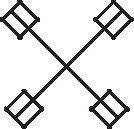
\includegraphics[width=0.1\textwidth]{%
gesamttex/edit_VIII,3/images/LH_38_212-215_d15_215r.pdf%
}} 
\vspace{0.5em}
\centerline{%
\lbrack\textit{Fig.~15}\rbrack%
}
% \newpage%
\vspace{1.5em}
%
%
\pstart
\edtext{}{%
\lemma{\hspace*{1,6mm}%
\lbrack\textit{Fig.~15}\rbrack%
}\killnumber%
\Cfootnote{%
tlw.\ Übernahme der Vorlage: a.a.O., Pl.~11, Fig.~154.\cite{01500}%
}}
%
\edtext{Par cette machine on trouve
%
\edtext{\lbrack\textit{les}\rbrack}{%
\lemma{}%
\Bfootnote{la %
\textit{L ändert Hrsg.}}} 
%
loix de l'\textit{equilibre de tous les corps comme par la precedente}, 
%
2\textsuperscript{do} on deduit \textit{tous les chocs possibles du seul equilibre}, 
%
3\textsuperscript{o} on reduit \textit{tous les chocs possibles à l'equilibre.}}{%
\lemma{Par \lbrack...\rbrack\ \textit{l'equilibre}}%
\Cfootnote{a.a.O., S.~426f.\cite{01500}}} 
%
(\protect\vphantom)+ Ce n'est que pour deux corps, ma
%
\edtext{maniere en}{\lemma{maniere}\Bfootnote{\textit{(1)} dans \textit{(2)} en \textit{L}}}
%
\edtext{suspendant plusieurs corps d'une}{\lemma{suspendant}\Bfootnote{\textit{(1)} des corps \textit{(2)} plusieurs corps \textit{(a)} dans \textit{(b)} d'une \textit{L}}} 
%
voute haute seroit plus parfaite. En les faisant decrire des cycloides\protect\index{Sachverzeichnis}{cycloide} on seroit encor maistre du temps du concours. En les lachant ensemble, ils viendroient ensemble à l'horison. \lbrack+\protect\vphantom()\rbrack
\pend
\count\Bfootins=1200%
\count\Afootins=1200%
\count\Cfootins=1200 
%